
\documentclass[a4paper, 12pt, twoside, headsepline=true]{scrartcl} % headsepline ist für die Linie unter der Kopfzeile verantwortlich

% Package für Sprachformatierung und Spellchecks
% http://ctan.space-pro.be/tex-archive/macros/latex/contrib/polyglossia/polyglossia.pdf
\usepackage{polyglossia}
\setdefaultlanguage[spelling=new]{german}

% Package zum Ändern von Headern & Footers
% mirrors.ctan.org/macros/latex/contrib/koma-script/doc/scrguien.pdf
\usepackage[automark]{scrlayer-scrpage}
\clearpairofpagestyles
\ihead{\headmark}
\ohead{\pagemark}

\pagestyle{scrheadings}
\setkomafont{pageheadfoot}{\small}

% Package zum Festlegen von Zeilenabstand
% https://www.namsu.de/Extra/pakete/Setspace.html
\usepackage[onehalfspacing]{setspace}
\setmainfont{Charis SIL} % set the main body font (\textrm), assumes Charis SIL is installed
\setlength{\parindent}{0pt}


\usepackage{csquotes}

% Package für das Referenzieren von Quellen aus .bib-Datei
\usepackage[style=ieee]{biblatex}
\addbibresource{mybib.bib}

% Package zum "Patchen" von Befehlen
% http://vesta.informatik.rwth-aachen.de/ftp/pub/mirror/ctan/macros/latex/contrib/xpatch/xpatch.pdf
% Überschreibt biblatex-Funktionalität, damit keine leeren Jahresklammern gedruckt werden
\usepackage{xpatch}
\xpatchbibdriver{online}
{\printtext[parens]{\usebibmacro{date}}}
{\iffieldundef{year}
	{}
	{\printtext[parens]{\usebibmacro{date}}}}
{}
{\typeout{There was an error patching biblatex-ieee (specifically, ieee.bbx's @online driver)}}

% Package zum Anpassen von enumerations-items 
% https://de.wikibooks.org/wiki/LaTeX-W%C3%B6rterbuch:_enumitem
\usepackage{enumitem}
\renewcommand{\labelitemiii}{$\star$}

% Package für die Anpassung der Seitengestaltung, z.B. Seitenränder
% https://www.namsu.de/Extra/pakete/Geometry.html
\usepackage{geometry}

% Package für Tabellengestaltung mit horizontalen Trennlinien
% https://www.namsu.de/Extra/pakete/Booktabs.html
\usepackage{booktabs}

% Package für Gestaltung und Anpassung einzelner Tabellenzellen 
% http://babyname.tips/mirrors/ctan/macros/latex/contrib/makecell/makecell.pdfx
\usepackage{makecell}

% Package für Positionierung von "floats", also nichtfesten Elementen wie Tabellen oder Bildern, die sich je nach Textgestaltung verschieden auf der Seite befinden müssen
% http://vesta.informatik.rwth-aachen.de/ftp/pub/mirror/ctan/macros/latex/contrib/float/float.pdf
\usepackage{float}

% Package für Tabellengestaltung 
%siehe https://www.namsu.de/Extra/pakete/Ltxtable.html
\usepackage{ltxtable}
\usepackage{filecontents}

%Package zum horizontalen Zentrieren von Tabelleninhalten
\usepackage{array}
\newcolumntype{P}[1]{>{\raggedright\arraybackslash}p{#1}}

% Package zum Anpassen von Macros/KeyValue-Daten. Hab ich garnicht verwendet, glaube ich
% http://mirrors.ibiblio.org/CTAN/macros/latex/contrib/adjustbox/adjustbox.pdf
\usepackage[export]{adjustbox}

% Package für Verwaltung von Acronymen 
% https://www.namsu.de/Extra/pakete/Acronym.html
\usepackage[printonlyused]{acronym}

% Package zum Implementieren von Textlinks
% https://www.namsu.de/Extra/pakete/Hyperref.html
\usepackage[
german,
colorlinks=true,
linkcolor=blue, % einfache interne Verknüpfungen
%TODO: Folgende Zeile für Druckdokument verwenden!
%hidelinks=true
anchorcolor=black,% Ankertext
citecolor=green, % Verweise auf Literaturverzeichniseinträge im Text
urlcolor=cyan % Farbe der URLs
%Back-Links zu den Kapiteln
]{hyperref}
\apptocmd{\UrlBreaks}{\do\f\do\m}{}{}
\setcounter{biburllcpenalty}{9000}% Kleinbuchstaben
\setcounter{biburlucpenalty}{9000}% Großbuchstaben
\setcounter{biburlnumpenalty}{9000}% Zahlen
%\usepackage[german,draft]{hyperref}

%Neudefinition für den Name von Subsubsection, damit "Unterunterabschnitt" nicht bei Referenzen auftaucht
\def\subsubsectionname{Unterabschnitt}%
\def\subsubsectionautorefname{Unterabschnitt}%

% Package für besseren Umgang mit Grafiken
% http://ftp.gwdg.de/pub/ctan/macros/latex/required/graphics/grfguide.pdf
\usepackage{graphicx}

% Package für Platzieren von Bildern neben/im Text
% https://www.namsu.de/Extra/pakete/Wrapfig.html
\usepackage{wrapfig}
\newcommand{\myhline}{\noalign{\global\rulewidth0,1cm}\hline
	\noalign{\global\arrayrulewidth1pt}}
% Umbenennung der Caption Beschreibung unter Bildern von "Abbildung" in "Abb." um Platz zu sparen.
\addto\captionsgerman{%
	\renewcommand{\figurename}{Abb.}%
}

% Definiere eine neue Liste bei der die Unterpunkte auch nummeriert sind, wie bei einem Inhaltsverzeichnis.
\newlist{legal}{enumerate}{10}
\setlist[legal]{label*=\arabic*.}
%\setcounter{tocdepth}{4}
%\setcounter{secnumdepth}{4}

\makeatletter 
\@addtoreset{figure}{section} 
\@addtoreset{table}{section} 
\makeatother 

%Commands zum Neustarten der Seitennummerierung ab Inahltsverzeichnis, falls vorher noch Titelseiten o.Ä. folgen
\renewcommand{\thefigure}{\thesection.\arabic{figure}} 
\renewcommand{\thetable}{\thesection.\arabic{table}} 

\begin{document}
% Nötig um in der PDF Datei einen Lesezeicheneintrag für das Inhaltsverzeichnis zu bekommen.
\pdfbookmark[1]{Inhaltsverzeichnis}{toc}
\tableofcontents
\clearpage
\newpage

\addsec{Abkürzungsverzeichnis}

\pdfbookmark[2]{Abkürzungsverzeichnis}{toc}
% Angabe in eckigen Klammern sollte das längste Acronym enthalten.
% Das ist notwendig damit sich der Einschub am längsten Acronym orientiert.
\begin{acronym}[header=Abkürzungsverzeichnis]
	\acro{arm}[ARM]{Architectural Reference Model}
	\acro{bpd}[BPD]{Business Process Diagram}
	\acro{bpel}[BPEL]{Business Process Execution Language}
	\acro{bpm}[BPM]{Business Process Management}
	\acro{bpmn}[BPMN]{Business Process Model and Notation}
	\acro{bpmn4cps}[BPMN4CPS]{Business Process Model and Notation for Cyber-Physical Systems}
	\acro{bpms}[BPMS]{Business Process Management System/Suite}
	\acro{cmmn}[CMMN]{Case Management Model and Notation}
	\acro{cps}[CPS]{Cyber-Physical Systems}
	\acro{ecaa}[ECAA]{Event Condition Action Alternative Action}
	\acro{eepk}[eEPK]{erweiterte Ereignisgesteuerte Prozesskette}
	\acro{eoi}[EoI]{Entity of Interest}
	\acro{gdv}[GDV]{Gesamtverband der Deutschen Versicherungswirtschaft}
	\acro{iapmc}[IAPMC]{IoT-aware Process Modelling Concept}
	\acro{ibpms}[iBPMS]{intelligent Business Process Management System/Suite}
	\acro{iot}[IoT]{Internet of Things}
	\acro{iota}[IoT-A]{Internet of Things - Architecture}
	\acro{m2m}[M2M]{Machine-to-Machine}
	\acro{nfc}[NFC]{Near Field Communication}
	\acro{omg}[OMG]{Object Management Group}
	\acro{p2m}[P2M]{Person-to-Machine}
	\acro{rfid}[RFID]{Radio-frequency Identification}
	\acro{uml}[UML]{Unified Modelling Language}
\end{acronym}

\clearpage

\addcontentsline{toc}{section}{Tabellenverzeichnis}

\listoftables

\clearpage

\addcontentsline{toc}{section}{Abbildungsverzeichnis}
\listoffigures
\clearpage


\section{Einleitung} \label{sec:section}
%TODO Einleitung muss am Ende besser an den Inhalt angepasst werden
Ziel dieser Thesis ist die Konzeption eines Modellierungsansatzes für \ac{iot}
Workflows. Hierfür werden grundlegende Besonderheiten von \ac{iot} Workflows festgehalten und davon ausgehend Evaluierungskriterien für die Bewertung gängiger Modellierungsansätze abgeleitet. Anhand der Kriterien werden Modellierungsmethoden bewertet und mögliche Erweiterungsmöglichkeiten vorgestellt. Der daraus resultierende Ansatz wird auf vorhandene Use-Cases angewandt und bewertet.

\subsection{Motivation} \label{motivation}
Das \ac{iot} ist eines der größten IT-Buzzwords der letzten Jahre und beschreibt die durch eingebettete Elektronik ermöglichte Vernetzung von physischen Dingen. Die dadurch gewonnen Daten bzw. Ereignisse, bieten neben dem Potential der Prozessoptimierung und Erweiterung die Möglichkeit zur Generierung völlig neuer Geschäftsprozesse und Modelle. 
Das Weiteren sinken die Kosten physische Dinge mit Sensoren auszustatten und untereinander zu vernetzen, was zu einer hohen Anzahlvon \ac{iot} Projekten führt. Laut Gartner sollen im Jahr 2020 mehr als die Hälfte der wichtigsten Geschäftsprozess Elemente des \ac{iot} beinhalten \cite{garnteriotgrowth}. Da der Wettbewerb auf dem Technologiemarkt rasant zu nimmt, ist es unerlässlich sich von der Konkurrenz abzuheben. Die Verwaltung von IoT Geräten, sogenannten Smart Devices, mit \ac{bpm} ermöglicht eine einfache Wartung ihrer Orchestrierung. Des weiteren bietet es die Möglichkeit der Nachverfolgung, die es erlaubt KPIs über die Prozesse und Devices einfach zu ermitteln. Diese KPIs sind maßgebend für ein effektives Arbeiten mit der stetig wachsenden Anzahl von Devices \cite{bpmofthings}. 

\subsection{Problemstellung} 
Während sich das IoT im Allgemeinen auf Kommunikation und Datenfluss konzentriert, berücksichtigen \ac{bpm}-Ansätze den Kontrollfluss, große monolithische Prozessmodelle und asynchrone Interaktionen. Darüber hinaus haben die meisten BPM-Ansätze Probleme mit nicht routinemäßigen, nicht deterministischen Prozessen, während IoT-Anwendungen typischerweise solche Interaktionen beinhalten. Das Problem der Vereinigung von \ac{iot} und \ac{bpm} beginnt bereits bei der Darstellung und Modellierung der neuen Geschäftsprozesse, da Standards wie \ac{bpmn} nur bedingt hierfür geeignete Elemente vorsehen. Das aufkommen der überwältigenden Datenmenge sorgt dafür, dass Objekte selbständige Routinen, sogenannte Verhaltensmuster oder Gewohnheiten ausführen. Dieses selbständige Handeln ohne zentrale Steuerung macht die Modellierung umfassender End-to-End Prozesse praktisch unmöglich. Dementsprechend müssen diese Verhaltensmuster als sogenannte event-driven micro processes organisiert werden. Da die Wechselwirkungen zwischen diesen Mikroprozessmodellen nicht auf der niedrigen Ebene des Nachrichtenaustausches beschrieben werden können, müssen diese laut "The Internet-of-Things Meets Business Process Management: Mutual Benefits and Challenges" auf einer höheren semantischen Ebene beschrieben werden \cite{iotmeetsbpm}. Diese Problemstellungen bilden die Grundlage für diese Thesis.
%TODO Quelle zu event driven Microprocesses eventuell mit Bild, Wichtigkeit des Modells für die umsetzung von Geschäftsprozess in Workflow herausheben
%event driven microprocesses erklären

\subsection{Aufbau der Thesis}
Nach der Einleitung mit Motivation, Problemstellung, Zielsetzung sowie dem Aufbau der Thesis folgen Grundlagen im Bereich des \ac{iot}, der Prozess Modellierung sowie des \ac{bpm}, welche zum Verständnis der weiteren Arbeit dienen.
 
 Im Hauptteil werden typische Muster von \ac{iot} Workflows identifiziert. Aus den Mustern werden Unterschiede und Besonderheiten zwischen \ac{iot} Workflows und Workflows ohne \ac{iot} Integration herausgearbeitet, welche bei der Modellierung zu berücksichtigen sind. Folgend werden die bestehenden Modellierungskonzepte \ac{iota} und \ac{bpmn4cps} vorgestellt.
 Anhand der Unterschiede werden Evaluierungskriterien für die Geschäftsprozess Modellierung abgeleitet. Diese Evaluierungskriterien werden im Anschluss dazu verwendet um bestehende Modellierungsmethoden auf ihre Eignung zur Modellierung von \ac{iot} Workflows zu bewerten. Basierend auf der Bewertung wird ein Modellierungskonzept für \ac{iot} Workflows erarbeitet. Zur Evaluierung werden mehrere Use-Cases analysisiert und das entwickelte Modellierungskonzept darauf angewandt. Anhand der Ergebnisse wird das Modellierungskonzept bewertet.
 
Im Schlussteil wird das Ergebnis festgehalten, ein Fazit getroffen und weiterführende Arbeiten sowie ein Ausblick vorgestellt.
 
\newpage

\section{Grundlagen}
In diesem Kapitel werden zunächst Grundlagen des \ac{iot} erläutert. Anschließend werden die wichtigsten Modellierungsmethoden für Prozesse dargestellt und Grundlagen des \ac{bpm} erklärt. Zum Abschluss werden zwei Erweiterungen von \ac{bpmn} zur Modellierung von \ac{iot} Workflows vorgestellt.

\subsection{BPM}
Laut der Defintion von bpm.com, der größten Internetseite im Bezug auf Artikel, Nachrichten, Forschung und Veröfftentlichungen für \ac{bpm} \cite{aboutbpmcom} versteht sich \ac{bpm} als: "eine Disziplin, die eine beliebige Kombination aus Modellierung, Automatisierung, Ausführung, Kontrolle, Messung und Optimierung von Geschäftsabläufen zur Unterstützung von Unternehmenszielen, übergreifenden Systemen, Mitarbeitern, Kunden und Partnern innerhalb und außerhalb der Unternehmensgrenzen umfasst"\cite{whatisbpm}. \ac{bpm}, in seinem Kern, nutzt den Workflow, um große Daten- und Informationsmengen zu verwalten, zu aktualisieren und zu verfolgen \cite{bpmofthings}. \\

\ac{bpm} setzt sich aus den in Abbildung \ref{bpmlifecycle} zu sehenden Phasen zusammen, Design, Modeling, Execution, Monitoring und Optimization. Im Zuge dieser Thesis wird der Augenmerk auf den Design und Modeling Aspekt des \ac{bpm} Lebenszyklus gelegt. Auf diese Aspekte wird in den Kapiteln \ref{modellierungsansätze} und \ref{anwendung} eingegangen \\
Besonders von einander zu Unterscheiden sind die Begriffe \ac{bpm} und \ac{bpms}. \ac{bpm} ist eine Praktik und kein Produkt. \ac{bpms} sind Produkte zum Beispiel von IBM oder Camunda. Was in den Produkten angeboten wird, hängt immer von Verkäufer des Produktes ab. \ac{bpms} sind dafür entworfen um \ac{bpm} zu unterstützen aber bieten darüber hinaus Funktionaltiäten welche nichts mit \ac{bpm} an sich zu tun haben.
Was genau die Kernfunktionalitäten eines \ac{bpms} sind wird im nächsten Unterkapitel beschrieben.

\begin{figure}[H]
	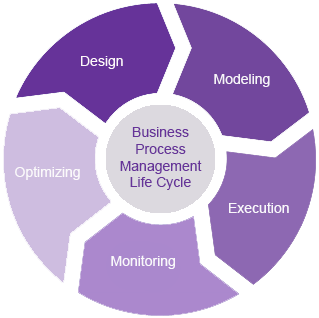
\includegraphics[height=5.5 cm,keepaspectratio,center]{figures/BPMLifecycle}
	\caption{BPM Lebenszyklus \cite{bpmlifecycle}}
	\label{bpmlifecycle}
\end{figure}


\subsubsection{BPMS}
Wie zuvor beschrieben sind \ac{bpms} dafür entworfen um die \ac{bpm} zu unterstützen. Folglich können alle Informationssysteme, die sich mit der Definition, Verwaltung, Anpassung und Bewertung von Aufgaben befassen, welche sich aus Geschäftsprozessen und Organisationsstrukturen ergeben als \ac{bpms} bezeichnen. Diese Produkte sind in der Lage, den Workflow in einer Organisation zu definieren, zu steuern, Daten zu übertragen und alte Informationssysteme, bestehende Programme und Programmmodule zu integrieren \cite{bpms}. Das Gebiet der \ac{bpms} besitzt 2017 einen geschätzten Marktwert von 14,5 Milliarden USD und lässt sich auf die grossen Anteilshaber wie IBM, Pegasystems und RedHat zurückführen \cite{bpmsmarket}.

\subsubsection{iBPMS}
Der Begriff \ac{ibpms}  wurde von Gartner geprägt und kann als natürliche Weiterentwicklung der \ac{bpms} verstanden werden. \ac{ibpms} bieten durch zusätzliche Funktionen wie zum Beispiel die Integration mit Social Media, mobile Prozessaufgaben, Streaming-Analysen sowie Echtzeit-Entscheidungsmanagement mehr "Intelligenz" in Geschäftsprozessen \cite{onibpms}.  In Tabelle \ref{table:GartnerIBPMS} werden die Kernfunktionalitäten von \ac{ibpms} und deren Erklärung dargestellt. Der Begriff \ac{ibpms} wurde von  \ac{bpms} Herstellern wie Pegasystems und Appian angenommen und in ihr Portfolio übernommen \cite{appianibpms} \cite{pegaibpms}.

\begin{filecontents}{\jobname-iBPMSTable.tex}
	\begin{longtable}{P{4cm}|X}
		\caption{Kernfunktionalitäten eines iBPMS \cite{ibpms}}\\
		\label{table:GartnerIBPMS}
		% Definition des ersten Tabellenkopfes auf der ersten Seite
		\textbf{Funktionalität} & \textbf{Erklärung}  \\ \hline
		\endfirsthead % Erster Kopf zu Ende
		%  Definition des Tabellenkopfes auf den folgenden Seiten
		\textbf{Funktionalität} & \textbf{Erklärung}  \\ \hline
		\endhead % Zweiter Kopf ist zu Ende
		% Ab hier kommt der Inhalt der Tabelle
		Interaktions-management & Die Funktionalität, verschiedene Arten von Aktivitäten und Interaktionen zur Laufzeit zu orchestrieren, um die Arbeit zu unterstützen, welche von Menschen, Systemen und Dingen (wie im \ac{iot}) geleistet wird, um spezifische Geschäftsergebnisse zu erzielen.\\ \hline
		Hochproduktive App Generierung & Ermöglicht IT-Entwicklern, schnell und einfach eine prozessorientierte Anwendung zu erstellen.
		Anwendungen, die auf der Plattform basieren, verwenden ein Metadatenmodell, um den gesamten Lebenszyklus von Geschäftsprozessen zu verwalten und prozessbezogene Daten zu bearbeiten.\\ \hline
		Überwachung und Geschäftsanpassung & iBPMS Plattformen unterstützen Business Activity Monitoring um den Status von Prozessinstanzen, Fällen und anderen Verhaltensweisen in nahezu Echtzeit kontinuierlich zu überwachen.\\ \hline
		Regeln und Entscheidungs Management &  Softwaresysteme wie inference engines, recommendation engines und decision management capabilities, die als Orientierungshilfe dienen, um menschliche oder automatisierte betriebliche Entscheidungen nach Geschäftsrichtlinien zu treffen.\\ \hline
		Analysen & \ac{ibpms} wenden müssen Logik und Statistiken auf Daten anwenden, um Erkenntnisse für bessere Entscheidungen zu gewinnen. Ein \ac{ibpms} kann prädiktive Analysen wie z.B. Scoring Services oder präskriptive Analysen wie z.B. optimization engines enthalten oder mit diesen in Verbindung stehen.\\ \hline
		Kompatibilität &  Kompatibilität mit externen Anwendungsdiensten und Systemen muss gewährleistet sein. Zu diesen Diensten und Systemen gehören benutzerdefinierte und kommerzielle Standardanwendungen sowie Cloud-basierte SaaS-Anwendungen und deren Datenbanken.\\ \hline
		Mobile Verwendbarkeit & Die Möglichkeit, von einer Vielzahl mobiler Geräte, einschließlich Smartphones und Tablets, auf Anwendungen zuzugreifen. Die Plattform bietet nicht nur Zugriff von jedem Ort aus, sondern optimiert auch die nativen Fähigkeiten des Mobilgeräts, einschließlich der Kamera und anderer Sensoren.\\ \hline
		Kontext- und Verhaltensstatistik & Die Fähigkeit der Plattform verkürzt die Zeit, welche benötigt wird, um Verhaltensweisen die zur Verbesserung der Geschäftsergebnisse erforderlich sind zu erkennen und zu optimieren. Dies kann die Analyse der vergangenen Ausführungshistorie oder die Simulation von Verhaltensvorschlägen beinhalten.\\
	\end{longtable}
\end{filecontents}
\LTXtable{\textwidth}{\jobname-iBPMSTable.tex}

Auch wenn \ac{ibpms} Interaction Management als eines seiner Kernfunktionalitäten besitzen muss, ist hier kein Standard für die Modellierung von \ac{iot} Workflows gegeben beziehungsweise vorgegeben. Es bleibt jedem Hersteller selbst überlassen wie die Worfklows zu modellieren sind.

\subsection{Internet of Things}
Die Idee eines Internets der Dinge hat seine Ursprünge in den Konzepten des Anfang der 90er Jahre von Mark Weiser skizzierten "Ubiquitous Computing". Dies bezeichnet er als nahtlose Einbindung von Computern in die reale Welt bezeichnet \cite{ucweiser}. \\
Grundgedanke des "Ubiquitous Computing" ist eine Erweiterung beliebiger physischer Gegenstände über ihre bestehende Form und Funktion hinaus durch mikroelektronische Komponenten \cite{237456}. Die so entstehenden "smarten" Gegenstände bilden, mit digitaler Logik, Sensorik und der Möglichkeit zur Vernetzung ausgestattet, ein Internet der Dinge.\\
 Der Begriff \acl{iot} wurde jedoch erst 1999 von Kevin Ashton im Zusammenhang eines globalen Netzwerks aus Objekten welche mit RFID angereicht wurden bei einer Präsentation bei Procter \& Gamble erstmals verwendet \cite{rfidiot}. \\
 Eine einheitliche Definition des \ac{iot} gibt es nicht, diese Thesis beruht auf der 2012 publizierten Definition aus "Overview of the IoT" der International Telecommunication Union. Diese definiert \ac{iot} als :"Eine globale Infrastruktur für die Informationsgesellschaft, die fortschrittliche Dienste ermöglicht, indem sie (physische und virtuelle) Dinge miteinander verbindet, die auf bestehenden und sich entwickelnden interoperablen Informations- und Kommunikationstechnologien basieren" \cite{iotdefinition}. \\
Aus technischer Sicht steht hinter dem Internet der Dinge weniger eine einzelne Technologie oder eine spezifische Funktionalität als vielmehr ein Funktionsbündel. Dieses Funktionsbündel lässt in seiner Gesamtheit eine neue Qualität der Informationsverarbeitung entstehen und ermöglicht somit neue Geschäftsmodelle.

\subsubsection{Smart Objects}
 Die in Tabelle \ref{table:smartObjectsCharacteristics} sichtbaren charakteristischen Merkmale definieren "smarte" Objekte welches die Grundlage des \ac{iot} bilden.

\begin{filecontents}{\jobname-smartObjectsTable.tex}
	\begin{longtable}{P{4.5cm}|X}
		\caption{Charakteristiken von "smarten" Objekten\cite{iotwiki}}\\
		\label{table:smartObjectsCharacteristics}
		% Definition des ersten Tabellenkopfes auf der ersten Seite
		\textbf{Charakteristik} & \textbf{Erklärung}   \\ \hline
		\endfirsthead % Erster Kopf zu Ende
		%  Definition des Tabellenkopfes auf den folgenden Seiten
		\textbf{Charakteristik} & \textbf{Erklärung}  \\ \hline
		\endhead
		% Ab hier kommt der Inhalt der Tabelle
		Identifikation & Objekte im Internet der Dinge sind über einen Schlüssel eindeutig identifizierbar. Diese Identifikation ermöglicht die Verknüpfung des Objekts mit Diensten, welche Informationen des physischen Objektes auf einem Server bereitstellen. \\ \hline
		Kommunikation & Im Gegensatz zu herkömmlichen phyischen Objekten verfügen Objekte im Internet der Dinge über die Möglichkeit Ressourcen im Netz oder sogar untereinander zur Verfügung zu stellen, um Daten und Dienste gegenseitig zu nutzen.\\ \hline
		Sensorik & Das "smarte" Objekt sammelt Informationen über seine Umwelt (Temperatur, Lichtverhältnisse, Luftdruck usw.), zeichnet diese auf und/oder reagiert darauf.\\ \hline
		Lokalisierung & Smarte Objekte kennen ihren Aufenthaltsort oder sind für andere lokalisierbar, beispielsweise auf globaler Ebene durch GPS oder in Innenräumen durch Ultraschall .\\ \hline
		Speicher & Das Objekt verfügt über Speicherkapazität, so dass es beispielsweise Informationen über seine Vergangenheit mit sich tragen kann.\\ \hline
		Aktuatorik & Objekte im Internet der Dinge können unter Umständen selbständig Entscheidungen ohne übergeordnete Planungsinstanz treffen, zum Beispiel im Sinne eines Industriecontainers, der seinen Weg durch die Lieferkette selbst bestimmt.\\ \hline
	\end{longtable}
\end{filecontents}
\LTXtable{\textwidth}{\jobname-smartObjectsTable.tex}
%TODO Verbessern, ausführlicher auf die Differenzierung und dessen Auswirkung eingehen
Des Weiteren lassen sich diese "smarten" Objekte in die in Abbildung \ref{iotdevices} dargestellten Unterkategorien einteilen. "Dumb Devices" lassen sich als solche beschreiben welche lediglich in der Lage dazu sind eine bestimmte Art von Daten zu sammeln und bereit zu stellen wie zum Beispiel ein Thermometer oder Bewegungssensoren. "Semi intelligent" Devices sind neben dem sammeln sowie dem begrenzten Verarbeiten von Informationen ebenfalls auch in der Lage diese zu speichern. "Multi-Sensors Devices" sind hingegen in der Lage von mehreren Quellen stammenden Daten zu verarbeiten und lassen neben der \ac{m2m} Kommunikation auch das Eingreifen des Menschen mit \ac{p2m} Kommunikation zu. Sie fungieren also als eine Art "smart Gateway", Beispiel hierfür ist ein Raspberry PI. \\
Diese Aufteilung besitzt besondere Relevanz für diese Thesis, da die Fähigkeiten der Objekte maßgeblich die Modellierung der Prozesse beeinflusst. Je "schlauer" ein Device ist umso mehr Aufgaben können vom Device selbst übernommen werden.

\begin{figure}[H]
	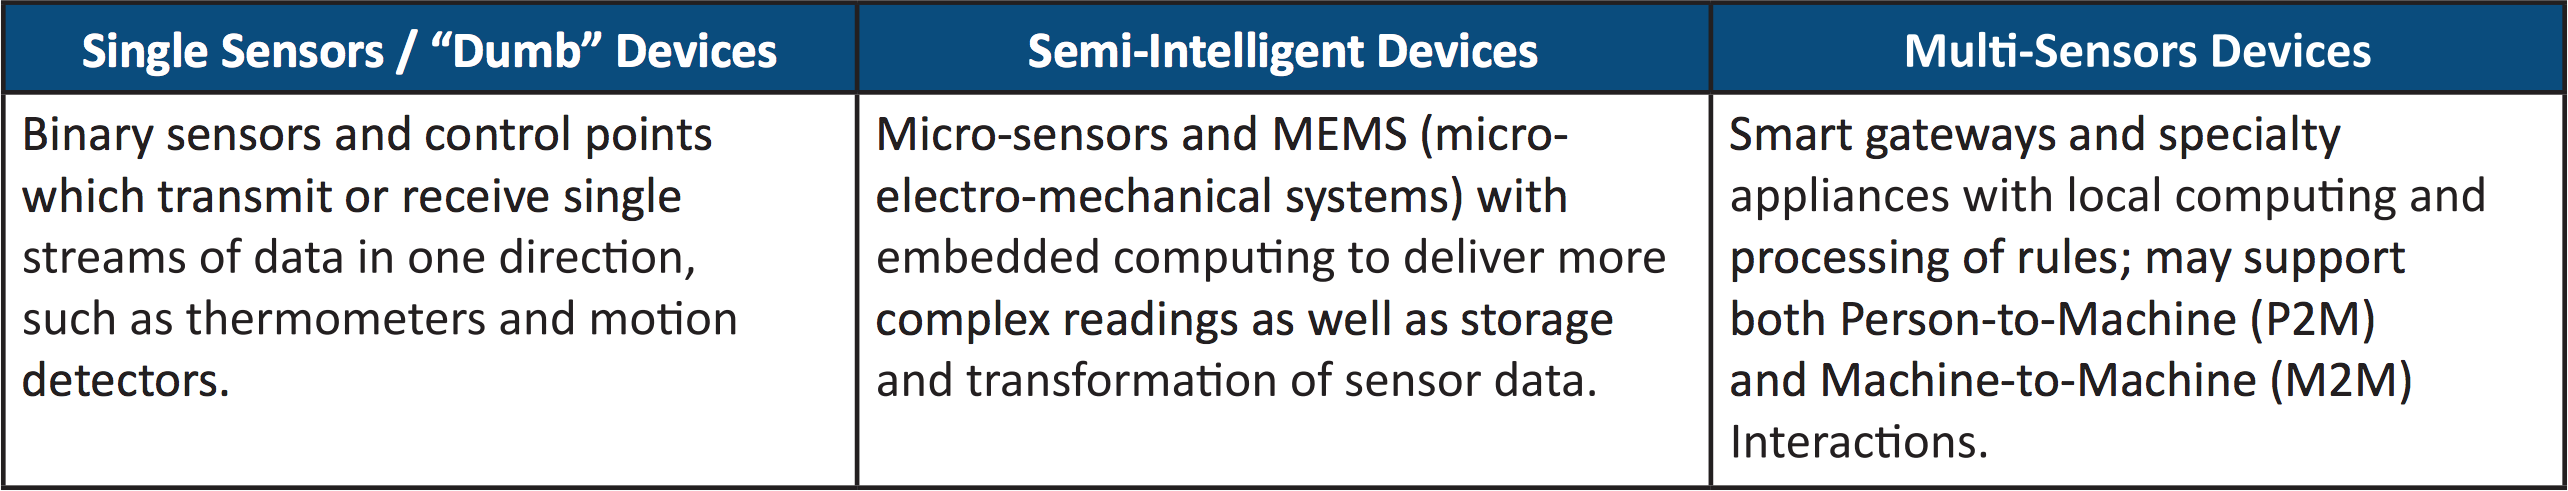
\includegraphics[height=3 cm,keepaspectratio,center]{figures/iotDevices}
	\caption{Unterschiedliche Arten der smarten Objekte \cite{iotdevices}}
	\label{iotdevices}
\end{figure}

\subsubsection{Domain Model}\label{sec:DomainModel}
Unter dem Buzzword \ac{iot} existieren sehr viele unterschiedlich Auffassungen und Interpretation wie beispielsweise das ursprüngliche Konzept Kevin Ashtons eines Netzwerkes aus um RFID angereicherter Objekte. Häufig ist auch von \ac{m2m} oder \ac{cps} die Rede. Bei dieser Vielzahl von Auffassungen und Begriffen ist es für ein allgemeines Verständnis unabdingbar sich auf eine Definition zu einigen. Im Zuge dieser Thesis wird das 2010 von Stephan Haller vorgestellte IoT Domain Model verwendet um den Zusammenhang zwischen Devices, Resourcen und Services zu erklären\cite{haller2010things}, da diese die am häufigsten genannte Quelle in der Literatur ist auf welcher diese Thesis beruht. Das Schaubild \ref{domainmodel} zeigt eine auf den Zusammenhang von Device, Service und Ressourcen abstrahierte Darstellung des IoT Domain Models. Im Anhang befindet sich ein Schaubild des vollständigen IoT Domain Models Haller´s vom Stand 2013.

\begin{figure}[H]
	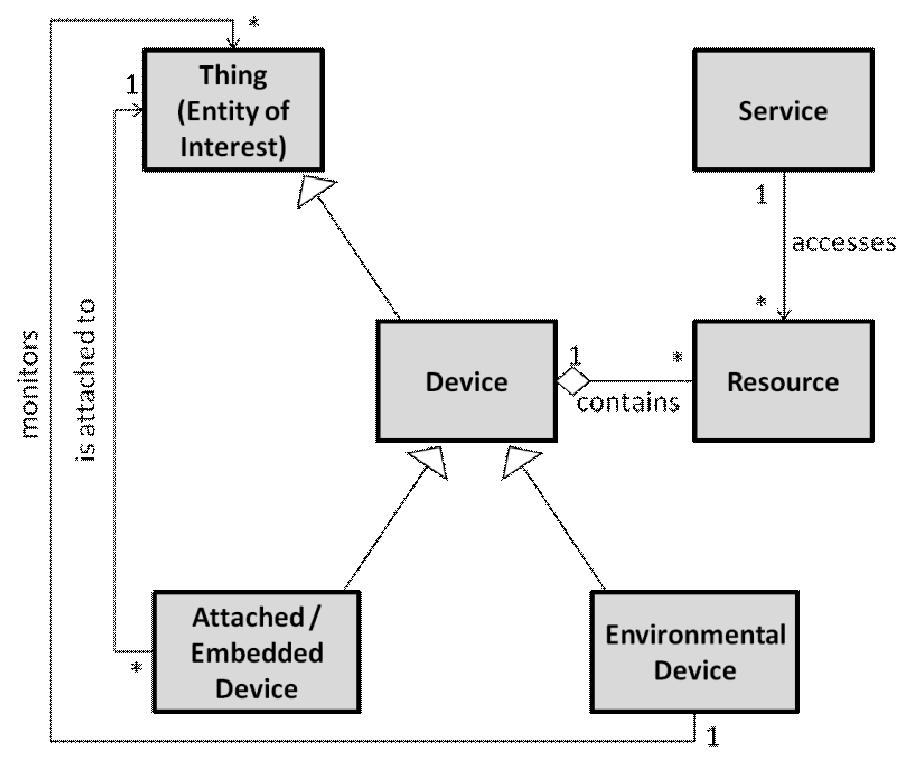
\includegraphics[height=8 cm,keepaspectratio,center]{figures/domainmodel}
	\caption{Zusammenhang zwischen Thing, Device, Resource und Service \cite{haller2010things}}
	\label{domainmodel}
\end{figure}

\textbf{Thing/ \ac{eoi}}: \\ 
Das \ac{eoi} bezeichnet einen physischen Gegenstand an welchem ein Nutzer oder eine Anwendung Interesse in Form von Informationen besitzt. Das \ac{eoi} wird entweder durch ein Environmental Device oder über ein oder mehrere "attached" beziehungsweise "embedded device" überwacht, welche am \ac{eoi} selbst angebracht sind.
\\

\textbf{environmental Device}: 
Environmental Devices, beziehungsweise Umgebungsgeräte überwachen und verfolgen den Status des \ac{eoi}. Hierbei überwachen Einvironmental Devices ein oder mehrere \ac{eoi}. Beispiele für Umgebungsgeräte sind \ac{rfid} Lesegeräte, Barcodescanner oder Kameras

\textbf{attached/ embedded Device}: 
Als attached/embedded Device stellen ähnlich wie die Umgebungsgeräte den Zustand und den Status des \ac{eoi} fest. Der Unterschied liegt hierbei daran, dass die attached/embedded Devices am \ac{eoi} selbst und nicht in der Umgebung angebracht sind. Beispiel hierfür sind Sensoren wie Thermometer oder Manometer.
\\

\textbf{Device}: \\
Das Device wird als Überklasse der "environmental Devices" sowie der "attached/ embedded Device" verstanden. Es sammelt Informationen über das \ac{eoi} und stellt diese über die Möglichkeit der Kommunikation mit IT-Systemen zur Verfügung.
\\

\textbf{Resource}: \\
Als Resource werden die vom Device bereitgestellten digitalen Informationen über den Zustand oder die Betätigungsfähigkeiten eines physischen Objektes bezeichnet.
\\

\textbf{Service}: \\
Services stellen die Ressourcen des Devices über eine klar definierte und standardisierte Schnittstelle bereit und stellen diese Anwendungen oder anderen Services zur Verfügung. Somit wird die Funktionalität als Arbeitseinheit einem Geschäftsprozess zur Verfügung gestellt.
\\
\\
Zusammenfassend lässt sich der Zusammenhang zwischen \ac{eoi}, Device, Service und Resource also wie folgend beschreiben. Ein physisches Objekte an welchem Interesse besteht, wird durch die Überwachung mittels ein oder mehrerer Sensoren beziehungsweise Umgebungsgeräten als Device in der virtuellen Welt dargestellt. Dieses Device enthält mehrere Ressourcen also Informationen welche wiederum durch standardisierte Schnittstellen, den Services zur Verfügung gestellt werden.

\subsection{Prozessmodellierung}\label{modellierung}
In heutigen Unternehmen unterstützen Informationssysteme nicht mehr nur das Geschäft, sondern sind ein integraler Bestandteil davon. Unternehmen machen Gebrauch von Informationstechnologie, wie zum Beispiel Enterprise Resource Planning Systemen. Wichtig ist hierbei, dass ihre Systeme so aufgebaut sind, dass sie die Unternehmen unterstützen in denen sie zum Einsatz kommen. Das Geschäft bestimmt letztlich die Anforderungen, welche die Informationssysteme definieren. Die Entwicklung von Software ohne ein angemessenes Verständnis des Kontextes, in welchem diese Software betrieben werden soll, ist nahezu unmöglich. Um ein solches Verständnis zu erlangen, ist es unerlässlich, dass man ein Geschäftsmodell definiert.\\
 Ein Modell ist eine vereinfachte Sicht auf eine komplexe Realität. Diese Abstraktion erlaubt es irrelevante Details zu vernachlässigen und den Fokus auf die Kernelemente zu legen. Effektive Modelle erleichtern zudem
Diskussionen zwischen verschiedenen Stakeholdern im Unternehmen. Sie ermöglichen es ihnen, sich auf die wichtigsten Grundlagen zu einigen und auf gemeinsame Ziele hinzuarbeiten.\\
Die Modellierung von Geschäftsprozessen ist als Mittel zur Analyse und zum Design von Software akzeptiert und etabliert. Die sich ständig weiterentwickelnden Modelle helfen den Entwicklern ihr Denken zu strukturieren und zu fokussieren. Die Arbeit mit den Modellen dient zum Verständnis der Geschäftsprozesse und erhöht dadurch das Bewusstsein für neue Möglichkeiten zur Verbesserung der Geschäftsprozesse.

\subsubsection{BPMN}\label{bpmngrundlagen}
\ac{bpmn} ist ein Standard für die Geschäftsprozessmodellierung, der eine grafische Notation zur Spezifikation von Geschäftsprozessen in einem \ac{bpd} auf Grundlage traditioneller Flussdiagrammtechniken bereitstellt \cite[S.222]{Aagesen2015}. Das Ziel von \ac{bpmn} ist es, die Geschäftsprozessmodellierung für technische Anwender und für Geschäftsanwender zugänglich zu machen,damit die Geschäftsprozessmodellierung eine Kommunikations- und Automatisierungsgrundlage bildet.\\
 Hierfür wird eine Notation bereitgestellt, welche für Geschäftsanwender intuitiv ist und dennoch komplexe Prozesssemantik abbilden kann. Die seit 2011 von der \ac{omg} vorgestellte \ac{bpmn} 2.0-Spezifikation bietet auch Ausführungssemantik sowie das Mapping zwischen den Grafiken der Notation und anderen Ausführungssprachen, insbesondere der \ac{bpel}. \ac{bpmn} ist so konzipiert, dass es für alle Beteiligten leicht verständlich ist. \\
Zu den Anwendern gehören Business-Analysten, welche die Prozesse erstellen und verfeinern, technische Entwickler, die für die Implementierung zuständig sind sowie Führungskräfte welche Prozesse überwachen und verwalten \cite{vonRosing2015433}. Im Anhang befindet sich ein Poster mit einer Übersicht über die wichtigsten Modellierungsmethoden von \ac{bpmn}. \\
\newline

\textbf{\ac{cmmn}}\\
Aufgrund der fehlenden Möglichkeit Flexibilität abzubilden beziehungsweise da nicht alle Möglichen Szenarien bekannt sind oder aufgrund der Kombinatorik nicht modelliert werden können, wurde 2014 von der \ac{omg} ein eigener Standard \ac{cmmn} verabschiedet welcher in der Lage ist flexible Prozesse abzubilden.\\
 Als Case werden Aktivitäten bezeichnet, welche sich nicht exakt wiederholen lassen. Cases sind von sich entwickelnden Umständen oder von Ad-hoc-Entscheidungen im Bezug auf bestimmte Situationen abhängig. Diese Ad-hoc-Entscheidungen werden von sogenannten Wissensarbeitern gefällt.\\
 Zu den Anwendungsfällen des Case Managements gehören die Antrags- und Schadensbearbeitung in der Versicherungsbranche, die Patientenversorgung sowie die medizinische Diagnose im Gesundheitswesen, Hypothekenbearbeitung im Bankwesen, Problemlösung in Call Centern, Wartung und Reparatur von Maschinen und Anlagen sowie die Konstruktion von Sonderanfertigungen\cite{cmmnomg} . \\
Laut Heise sei die Kombination von \ac{cmmn} und \ac{bpmn} sinnvoll um sowohl strukturierte als auch unstrukturierte Prozesse oder Teilprozesse sinnvoll abbilden zu können \cite{cmmnheise}.

%TODO DMN eventuell noch interessant


\subsubsection{UML}\label{uml}
 \ac{uml} ist eine grafische Sprache, die Artefakte verteilter Objektsysteme visualisiert, spezifiziert, konstruiert und dokumentiert \cite{Kleuker}. Es ist der am weitesten verbreitete Standard für Software-Architekten, um Geschäftsanwendungen zu spezifizieren.\\
 \ac{uml} wird vor allem für die objektorientierte Softwareentwicklung im Bereich des Software-Engineerings eingesetzt.
Die \ac{uml} wurde in den 90er Jahren als Modellierungssprache und Methodik zur Unterstützung der objektorientierten Programmierung entwickelt. Im Jahr 1997 wurde es als Standard von der \ac{omg} übernommen. Die ersten Versionen 1.X wurden 2005 durch die neu überarbeiteten Versionen 2.X ersetzt. Seit März 2015 befindet sich UML in der Version 2.5 \cite{omguml}. \ac{uml} bietet im Gegenteil zu \ac{bpmn} mehr als nur die reine Prozessmodellierung und ist in ihrer Gesamtheit sehr umfangreich.\\
Die Spezifikation allein ist über eintausend Seiten lang. Strukturiert wird \ac{uml} in vier Gruppen, den  Strukturdiagrammen, den Architekturdiagrammen, den Verhaltensdiagrammen und den Kommunikationsdiagrammen. \\
Im Zuge dieser Thesis wird wird ausschließlich auf \ac{uml} Aktivitätsdiagramme im Bezug auf Prozessmodellierung eingegangen.
%Weitere Quelle http://www.uml.ac.at/wp-content/uploads/teaching/05_Aktivitaetsdiagramm_Folien.pdf

\subsubsection{Geschäftsregeln}\label{businessrules}
Geschäftsregeln sind generell keine Modellierungsmethode, allerdings lassen Geschäftsprozesse sich als eine Reihe von Geschäftsregeln darstellen. Die unter bestimmten Bedingungen auszuführenden Aktivitäten und die sie auslösenden Ereignisse können in Beziehung zueinander gesetzt werden, sodass Prozesse auf der Grundlage von Geschäftsregeln beschrieben und ausgeführt werden können.\\
Die Prozessmodellierung mit Geschäftsregeln basiert auf den  ECAA-Regeln durch die drei Konstrukte Ereignis, Bedingung und Aktion sowie alternativer Aktion (Event,Condition,Action,Alternative Action). Diese Art der Modellierung eignet sich für kleine Prozessmodelle und müssen für größere Modelle auf die \ac{eepk} Notation übertragen werden \cite{businessrules}. 

\newpage

\section{IoT Workflows und deren Besonderheiten}
In diesem Kapitel sollen grundlegende Muster in \ac{iot} Workflows erkannt werden. Anhand der Muster werden Unterschiede zu regulären Workflows erstellt welche im Anschluss zu Anforderungen an die Modellierung von \ac{iot} Workflows zusammengefasst werden. \\
Als Workflow wird eine inhaltlich abgeschlossene sowie zeitlich und sachlich Zusammenhängende Folge von Funktionen bezeichnet. Durch den Workflow werden die Aufgaben, Verarbeitungseinheiten sowie deren Beziehungen zu einander festgelegt \cite{workflowgabler}. Ein Workflow kann also als die informationstechnische Umsetzung eines Geschäftsprozesses verstanden werden. \\
Der Lebenszyklus eines Worklows besteht aus der Modellierung, der Ausführung und Überwachung sowie der Analyse des Workflows. Die Modellierung bildet hierbei den ersten Schritt für die Umsetzung von Workflows, dies geschieht durch einen der in \ref{modellierung} vorgestellten Standards der Geschäftsprozessmodellierung. Diese Thesis beschränkt sich auf den Modellierungsaspekt des Workflow Lebenszykluses.\\
Gängige Modelleriungsmethoden sind jedoch nicht in der Lage die \ac{iot} spezifischen Besonderheiten welche für die Umsetzung eines Geschäftsprozesses in einen Workflow von großer Bedeutung sind darzustellen. Deshalb werden im Kapitel \ref{modellierungsansätze} Erweiterungen für die Modellierung von \ac{iot} Geschäftsprozessen vorgestellt.

%Mögliches Problem, Darstellung von Streams. Mögliche Lösung Time based Subprocesses mit IoT A modelliert,ermöglicht genaue zuweisung und nachverfolgung von IoT Device zu physical Entity -> wichtig für automatisierung (workflow). \\

\subsection{Schlüsselsektoren des IoT} \label{iotmuster}
Da das \ac{iot} eine noch sehr junge Technologie ist und sich größtenteils im experimentellem Stadium befindet existieren nur wenige Best Pracitices. Im 2017 erschienen "Review of latest developments in the Internet of Things" Bericht der Cambridge Consultants wurden die Schlüsselsektoren und Anwendungen von \ac{iot} identifiziert. Hierbei handelt es sich um zwölf Schlüsselsektoren und 168 Anwendungen\cite[S.24-26]{iotDevelopments}. Im Folgenden werden zehn Anwendungsgebiete analysiert um im Kapitel \ref{muster} daraus Typische Muster von \ac{iot} Workflows abzuleiten.

\subsubsection{Automobilbranche}
Automobile sind mit einer Vielzahl an Sensoren ausgestattet welche permanent Informationen über das Fahrzeug sammeln. Diese Daten können teilweise vom Fahrzeug selbst ausgewertet werden und bedürfen somit nicht die Verwendung von \ac{iot}, Beispiel hierfür ist das autonome Fahren. \ac{iot} findet  jedoch besonders im Bereich des automatisierten Notrufs eine Anwendung\cite[S.32-35]{iotDevelopments}. Die durch die Sensoren gesammelten Daten können durch Technologien wie Complex Event-Processing ausgewertet werden und dadurch Unfälle erkannt werden. Durch die Vernetzung des Fahrzeugs kann ein Notruf mit der aktuellen Position über das Fahrzeug an die zuständige Behörde weitergeleitet werden.

\subsubsection{Unterhaltungselektronik und schnelldrehende Konsumgüter}
Vernetzte Konsumgüter werden verwendet, um das Leben einfacher, produktiver oder erschwinglicher zu machen. Die Verbindung zum Internet  wird immer mehr zum Standard in der Unterhaltungselektronik.  Die gängigsten Beispiele hierfür sind Wearables, Smart Homes und Haushaltselektronik. Durch das Messen der Zustände der vernetzten Geräte und die Verfügbarkeit über das Internet ist der Verbraucher von überall dazu in der Lage seine Geräte zu verwalten\cite[S.37-41]{iotDevelopments}.

\subsubsection{Versorgung}
Die Europäpische Union begann schon 2009 damit die Einführung intelligenter Verbrauchsmessung voranzutreiben in dem sie sich vornahm 80\% der herkömmlichen Stromzähler bis 2020 durch intelligente Verbrauchsmesser zu ersetzen\cite[S.46-51]{iotDevelopments}. Der größte Nutzen hierbei ist eine bessere Verwaltung des Stromnetzes sowie Kosteneinsparungen, durch den Wegfall des Ablesens der Stromzähler. Hierbei wird lediglich der Verbrauch durch die Anbindung an das Internet automatisiert mitgeteilt.  Ein weiter Anwendungsfall ist die automatische Leckerkennung von Rohren, die durch das Messen des Wasserdrucks ermöglicht wird.

\subsubsection{Intelligente Städte}
Intelligente Städte könnten die Verwaltungskosten für den Staat reduzieren und die Lebensqualität ihrer Bewohner steigern. Schlüsselanwendungen sind hierbei Intelligente Beleuchtungskontrolle, Abfallmanagement sowie Verkehrsflusssteuerung\cite[S.51-57]{iotDevelopments}. \\Im Fall der Intelligenten Beleuchtungskontrolle könnten Laternen mit Lichtsensoren ausgestattet werden. Wenn Bedarf an Strom für die Beleuchtung einer Laterne besteht kann die Laterne das Beleuchtungssystem ansprechen und wird daraufhin mit Strom versorgt.\\
Mülleimer und Straßen könnten mit Sensoren beziehungsweise Chips ausgestattet werden um eine bedarfsbedingte Müllabholung zu ermöglichen. Sensoren in der Straße können einem zentralen Müllverwaltungssystem signalisieren, dass es Müll abzuholen gibt. Anhand der gesammelten Daten kann eine optimale Route der Müllabfuhr erstellt werden und somit Kosten gespart werden.\\
Durch das Sammeln von Verkehrsdaten kann eine bedarfsgesteuerte Ampelschaltung ermöglicht werden, was den Verkehrsfluss erhöht und Umweltbelastungen in den Städten durch Stau verringert. Hierbei werden die vom im öffentlichen Raum angebrachten Sensoren gesammelten Daten an ein Verkehrsverwaltungssystem gesendet welches diese auswertet. Ein weiterer Vorteil hierbei ist die Echtzeiterkennung von Unfällen wodurch eine schnellere Hilfeleistung ermöglicht wird und Verkehrsverhinderungen schnell beseitigt werden können.

\subsubsection{Fertigung}
Der Begriff Industrie 4.0 ist eines der größten Schlagwörter im Bezug auf \ac{iot}. Durch \ac{iot} verschmelzen die Grenzen zwischen dem Fabrikbetrieb, der Lieferkette und dem Produktdesign. Industrie 4.0 steht für das Versprechen einer vollautomatisierten Produktion von Individualprodukten. Hierbei werden Produkte mit \ac{rfid} Chips ausgestattet und sind jederzeit im Besitz über die Information zu welchem Bearbeitungsschritt sie als nächstes müssen. Jede Maschine teilt Informationen über ihren Zustand einem zentralen System mit und kann somit ideal gewartet werden. Des weiteren wird durch die Messung des Verbrauchs eine automatische Nachbestellung ermöglicht.

\subsubsection{Gesundheitswesen}
Im Gesundheitswesen bietet \ac{iot} die Möglichkeit die Versorgung von Patienten zu Verbessern\cite[S.68-72]{iotDevelopments}. \ac{iot} Devices ermöglichen eine permanente Überwachung des Zustandes von Patienten ohne, dass diese stationär aufgenommen werden müssen. Bei der Überschreitung von Grenzwerten kann direkt ein Notruf ausgelöst werden oder sogar zum Beispiel eine Injektion von Insulin durch ein weiteres Device auslösen.\\
Des weiteren lassen sich mithilfe der Daten über die Vitalfunktionen und anderer Werte die mithilfe von Wearables aufgezeichnet werden können, langfristig wissenschaftliche Erkenntnisse ziehen.

\subsubsection{Landwirtschaft und Umwelt}
 Durch das Ausstatten und Vernetzen von Gewächshäusern können im Bereich der Landwirtschaft sowohl Wasser und Energie gespart als auch Ernteerträge gesteigert werden \cite[S.74-75]{iotDevelopments}. Hierbei sammeln Sensoren Informationen über den Nährstoffgehalt des Trägerbodens, die Luftfeuchtigkeit, den Kohlenstoffdioxidanteil in der Luft welche dazu dienen um die unvorhersehbaren Auswirkungen des täglichen Betriebs zu erkennen und zu bewältigen.\\ Hierbei können sowohl die \ac{iot} Devices selbst einen Teil der Daten auswerten und eine Anpassung durch das ansprechen weiterer Devices veranlassen als auch eine langfristige Analyse durch zentrale Systeme gewährleisten.

\subsubsection{Bauwesen}
Der Hauptvorteil der Nutzung von IoT in der Baubranche liegt in der verstärkten Kontrolle über die Anlagen und Mitarbeiter. Dies ermöglicht eine Optimierung des gesamten Bauprozesses, was zu einer verbesserten Energienutzung, Ressourcenallokation und Anlagenverwaltung führt. \\
Hierbei wird \ac{iot} für die Überwachung von Spezialausrüstung für eine bessere Wartung sowie die Überwachung der Baustellen an sich verwendet um die Sicherheit der Mitarbeiter zu gewährleisten.

\subsubsection{Intelligente Gebäude}
Intelligente Gebäude versprechen eine bessere Energieeffizienz und mehr Bequemlichkeit für ihre Besitzer durch einen hohen Automatisierungsgrad\cite[S.82-85]{iotDevelopments}. Sensoren innerhalb des Hauses zeichnen Daten auf aus den sich Muster generieren lassen die den Alltag des Bewohners widerspiegeln. Dadurch lassen sich automatisierte Tagesabläufe ableiten. \\
Ein weiterer Anwendungsfall ist die Verbesserung der Sicherheit welche sich mit den verbauten Sensoren erreichen lässt. Wenn sich laut dem erstellten Tagesplan keine Person innerhalb des Hauses befinden sollte und dennoch ein Sensor Bewegungen wahrnimmt, dann kann das intelligente Haus seinen Besitzer darüber benachrichtigen.

\subsubsection{Einzelhandel und Freizeit}
Die derzeitigen Anwendungen konzentrieren sich hauptsächlich auf Anwendungen zur Kundenbindung und zur Effizienzsteigerung im Einzelhandel\cite[S.86-90]{iotDevelopments}. \\
Beispiel sind hierfür ist der automatisierte Checkout. Artikel sind mit \ac{rfid} Chips ausgestattet und werden sobald sie nahe der Kasse sind von Sensoren registriert. Somit kann eine Rechnung des Einkaufes über \ac{nfc} an das Smartphone gesendet und schnell und einfach bezahlt werden.

\subsection{IoT Workflows}\label{muster}
%TODO Text mit der Herleitung der Muster
Durch die in Kapitel \ref{iotmuster} analysierten Anwendungsfälle des \ac{iot} lassen sich die folgenden Muster abstrahieren.

Muster 1: Simpler \ac{iot} Worflow\\
Ein oder mehrere IoT Devices (Sensoren) überwachen den Zustand beziehungsweise Standort einer \ac{eoi}. Die Daten selbst können vom IoT Device ausgewertet werden. Bei Bedarf kann das Device andere Devices ansprechen.\\

Muster 2: Komplexer \ac{iot} Workflow\\
Die von den \ac{iot} Devices gesammelten Daten können nicht vom Decive selbst ausgewertet werden sondern werden an ein zentrales System gesendet, welches die Daten für die weitere Verwendung aufbereitet. Wenn es aufgrund der ausgewerteten Daten nötig ist in den Prozess einzugreifen, ist dieses System in der Lage dazu andere Devices anzusprechen. \\

Muster 3: Verwendung der \ac{iot} Daten \\ 
Durch \ac{iot} Devices werden große Mengen an Daten gesammelt. Diese Daten dienen dazu völlig neue Geschäftsmodelle zu kreieren wie zum Beispiel pay per Use. Hierbei können die von den IoT Device generierten Daten mittels Big Data Technologien wie maschinellem Lernen und Complex Event-Processing verwendet werden um aus den Datenmengen höherwertige Informationen und Ereignisse zu generieren.\\

Prozesse können aus ein oder mehreren Mustern zusammengesetzt werden.  

\subsection{Unterschiede IoT Workflows zu regulären Workflows}
Aus den in \ref{iotmuster} definierten Mustern von \ac{iot} Workflows lassen sich die \ac{iot}-spezifischen Unterschiede gegenüber regulärer Workflows ableiten. 

Der grundlegendste Unterschied von \ac{iot} Workflows liegt darin, dass \ac{iot} Devices einen neuen Akteur im Workflow darstellt, welcher Tätigkeiten ausführen und mit anderen Prozessteilnehmern sowie weiteren \ac{iot} Devices kommunizieren kann. \\
Eine Modellierung alleine als Akteur wird den Möglichkeiten aber nicht gerecht. Devices unterscheiden sich in ihren Eigenschaften von regulären Prozess Teilnehmern, sie können fest verbunden sein mit den Entitäten mit welchen sie zusammen arbeiten. Ein Device muss sich also ein oder mehrerer Entitäten zuweisen lassen. Diese Abhängigkeit ist bei der Modellierung zu berücksichtigen. \\
Durch die Verbundenheit von \ac{iot} Devices besitzen diese auch eine eigene Form mit Dingen innerhalb eines Prozesses zu interagieren, da ihre Handlungen sich im Kern auf den Zustand der ihr zugewiesen Entität beschränken.\\
Da sich die Entitäten innerhalb der Workflows bewegen können spielt Mobilität sowie die Fähigkeit den Standort der \ac{iot} Devices und Entitäten bestimmen zu können eine besondere Rolle in \ac{iot} Workflows\\
Die von den \ac{iot} Devices gesammelten Informationen unterscheiden müssen Metadaten darüber enthalten wann sie wo von welchem \ac{iot} Device über welche Entität gesammelt wurden sowie Aufschluss über die Qualität der Information selbst beinhalten um eine sinnvolle Auswertung der Informationen selbst zu ermöglichen.
IoT besitzt im Vergleich zu normalen Prozessen eine Vielzahl an öffentlichen Schnittstellen, daher spielt Security eine viel wichtigere Rolle als in normalen Geschäftsprozessen. Allerdings wird Security durch TOGAF  in den darunterliegenden Schichten Anwendungsarchitektur, Informationsarchitektur und Technologische Architektur umgesetzt \cite{enterpricearichitecture} und ist deshalb nicht bei der Modellierung selbst, sondern von der Software die diese Prozesse ausführt zu berücksichtigen.

\subsection{IoT Spezifische Anforderungen an die Modellierung}\label{anforderungen}
Aufgrund der Besonderheiten von \ac{iot} Workflows lassen sich spezifische Anforderungen beziehungweise Evaluierungskriterien für die Modellierung von IoT Workflows ableiten.

\begin{filecontents}{\jobname-Evaluerungskriterien.tex}
	\begin{longtable}{P{4.5cm}|X}
		\caption{Anforderung an IoT Modellierung}\\
		\label{table:evaluierungskriterien}
		% Definition des ersten Tabellenkopfes auf der ersten Seite
		\textbf{Anforderung} & \textbf{Erklärung}   \\ \hline
		\endfirsthead % Erster Kopf zu Ende
		%  Definition des Tabellenkopfes auf den folgenden Seiten
		\textbf{Anforderung} & \textbf{Erklärung}  \\ \hline
		\endhead % Zweiter Kopf ist zu Ende
		% Ab hier kommt der Inhalt der Tabelle
Device als Akteur & Devices müssen als neuer Akteur im Geschäftsprozess modellierbar sein.\\ \hline
Physische Dinge  & Informationen, Devices und Services müssen eindeutig physischen Dingen zuweißbar sein.\\ \hline
Spezielle Aufgabentypen & IoT Devices als Prozessteilnehmer benötigen eigene Aufgabentypen um ihren charakteristischen Merkmalen gerecht zu werden.\\ \hline
Informationen  & Die Informationen welche durch IoT Devices bereitgestellt werden müssen Metadaten über den Zeitpunkt, Ort, Herkunft ihrer Erstellung sowie über ihre Qualität besitzen.\\ \hline
Mobiltät & Prozessteilnehmer und Aktivitäten in IoT Prozessen sind ortsabhängig. Diese Abhängigkeit muss modellierbar sein.\\ \hline
Granularität & Prozesse müssen deutlich in mehrere Unterprozesse aufteilbar sein.\\
	\end{longtable}
\end{filecontents}
\LTXtable{\textwidth}{\jobname-Evaluerungskriterien.tex}
 
Diese spezifischen Anforderungen bilden die Grundlage für die im nächsten Kapitel stattfindende Evaluierung der \ac{iot} Modellierungskonzepte. Security ist zwar ein wichtiges Thema bei der Umsetzung eines \ac{iot} Geschäftsprozesses, wird jedoch bei der Modellierung n
 
\section{Betrachtung verschiedener Modellierungsansätze}\label{modellierungsansätze}
Obwohl IoT mittlerweile zum beliebten Schlagwort geworden ist, existieren immer noch Probleme mit dem Konzept, Prozesse auf \ac{iot} anzuwenden und diese fachgerecht darzustellen. In diesem Kapitel werden deshalb verschiedene Modellierungsansätze vorgestellt, welche auf die Besonderheiten von \ac{iot} Geschäftsprozesse spezialisiert sind.

\subsection{BPMN basierte Ansätze}
Eine Grundlegende Beschreibung zu \ac{bpmn} ist in Kapitel \ref{bpmngrundlagen} zu finden. Da sich nur Choreographie und Prozessdiagramme für die Darstellung für \ac{iot} Geschäftsprozesse eignen werden die restlichen \ac{bpmn} Diagrammtypen in dieser Thesis vernachlässigt.

\subsubsection{Choreographiediagramm}
\begin{filecontents}{\jobname-cdbewertung.tex}
	\begin{longtable}{P{4cm}|X}
		\caption{Umsetzung der IoT spezifischen Anforderungen durch BPMN Choreographiediagramme}\\
		\label{table:evaluierungskriterien}
		% Definition des ersten Tabellenkopfes auf der ersten Seite
		\textbf{Anforderung} & \textbf{Erklärung}   \\
		\hline
		\endfirsthead % Erster Kopf zu Ende
		%  Definition des Tabellenkopfes auf den folgenden Seiten
		\textbf{Anforderung} & \textbf{Erklärung}  \\
		\hline
		\endhead % Zweiter Kopf ist zu Ende
		% Ab hier kommt der Inhalt der Tabelle
		Device als Akteur & Aufgaben in Choreographiediagrammen besitzen immer einen initiierenden Teilnehmer und mindestens einen weiteren Teilnehmer. Je nachdem in welcher Rolle, also aktiver oder passiver Teilnehmer das Device agiert kann es sich dadurch in beiden Fällen darstellen lassen.\\ \hline
		Physische Dinge  & Physische Dinge lassen sich im Choreographiediagramm als passiver Prozessteilnehmer abbilden. Allerdings wird die Zugehörigkeit zwischen Device und physischen Ding hier nicht berücksichtigt und eine Zuweisung anhand der graphischen Notation ist nicht möglich. Der \ac{iot} spezifische Zusammenhang wird hierbei also nicht deutlich\\ \hline
		Spezielle Aufgabentypen & Choreographiediagramme besitzen keine besonderen Aufgabentypen. Die \ac{iot} spezifischen Aufgabentypen lassen sich dadurch also nicht darfstellen. \\ \hline
		Informationen  &  Informationen lassen sich nur in Form von Nachrichten darstellen. Diese Darstellung wird den Anforderungen nicht gerecht da die \ac{iot} spezifischen Merkmale nicht berücksichtig werden.\\ \hline
		Mobiltät & Es gibt keine Möglichkeit Prozessteilnehmer als mobil beziehungsweise Aufgaben als standortabhängig darzustellen.\\ \hline
		Granularität & Jeder Prozess kann aus einer Vielzahl von Unterprozesse dargestellt werden.\\
	\end{longtable}
\end{filecontents}
\LTXtable{\textwidth}{\jobname-cdbewertung.tex}

\subsubsection{Prozessdiagramm}
\textbf{Bewertung}
\\

\begin{filecontents}{\jobname-pdbewertung.tex}
	\begin{longtable}{P{4cm}|X}
		\caption{Umsetzung der IoT spezifischen Anforderungen durch BPMN Prozessdiagramme}\\
		\label{table:evaluierungskriterien}
		% Definition des ersten Tabellenkopfes auf der ersten Seite
		\textbf{Anforderung} & \textbf{Erklärung}   \\ \hline
		\endfirsthead % Erster Kopf zu Ende
		%  Definition des Tabellenkopfes auf den folgenden Seiten
		\textbf{Anforderung} & \textbf{Erklärung}  \\ \hline
		\endhead % Zweiter Kopf ist zu Ende
		% Ab hier kommt der Inhalt der Tabelle
		Device als Akteur & Devices lassen sich in \ac{bpmn} Prozessdiagrammen als Lane darstellen und sind in der Lage Tätigkeiten auszuführen.\\ \hline
		Physische Dinge  & Physische Dinge lassen sich als zugeklappter Pool darstellen. Die Zuweisung von Device zu physischem Ding lässt sich jedoch nur graphisch darstellen.\\ \hline
		Spezielle Aufgabentypen & Für die \ac{iot} spezifischen Aufgaben der Sensorik und Aktuatorik besitzt \ac{bpmn} keine geeigneten Elemente\\ \hline
		Informationen  & Die Informationen welche durch \ac{iot} Devices generiert werden können in \ac{bpmn} Prozessdiagrammen als DataObject dargestellt werden diese geben allerdings keine Auskunft über ihre Qualität, Herkunft oder Zeitpunkt der Erstellung. \\ \hline
		Mobiltät & \ac{bpmn} Prozessdiagramme bieten keine Möglichkeit Prozessteilnehmer oder Aufgaben als mobil oder standortabhängig zu kennzeichnen.\\ \hline
		Granularität & Jeder Prozess kann aus einer Vielzahl von Unterprozessen dargestellt werden.\\
	\end{longtable}
\end{filecontents}
\LTXtable{\textwidth}{\jobname-pdbewertung.tex}

\subsubsection{IoT - A}
\acl{iota} kann als eine Art Leuchtturmprojekt der Europäischen Union angesehen werden, welches 2013 nach über drei Jahren zu Ende ging. Ziel hierbei war es ein \ac{arm} als Grundlage für das \ac{iot} zu erstellen. Die Grundidee hierbei war, dass das \ac{arm} eine gemeinsame Struktur sowie Richtlinien für den Umgang mit Kernaspekten der Entwicklung, Nutzung und Analyse von \ac{iot}-Systemen bereitstellt, was eine nahtlose Integration heterogener \ac{iot}-Technologien in eine kohärente Architektur sowie den Zusammenschluss mit anderen Systemen des "Future Internet" ermöglicht \cite[S.17]{enablingthingstotalk}. Um dieses Ziel zu erreichen wurden einige detaillierte wissenschaftliche und technologische Zielsetzungen identifiziert welche innerhalb des Projektes behandelt werden\cite{meetiot}.\\


\textbf{Zielsetzungen}\\

1. Bewertung bestehender \ac{iot}-Protokoll Suites und Ableitung von Mechanismen zur Erzielung einer durchgehenden Interoperabilität für eine nahtlose Kommunikation zwischen \ac{iot}-Geräten. Das \ac{iot} wird aus Geräten mit unterschiedlichen Kommunikationsstacks bestehen. \ac{iota} soll einen nahtlosen Kommunikationsfluss zwischen heterogenen Geräten ermöglichen und dabei die Komplexität der End-to-End-Heterogenität vor dem Kommunikationsdienst verbergen.\\

2. Entwicklung von Modellierungswerkzeugen und einer Beschreibungssprache für zielorientierte \ac{iot}-bewusste (Geschäfts-)Prozessinteraktionen, die es erlauben, ihre Abhängigkeiten für eine Vielzahl von Bereitstellungsmodellen auszudrücken.\\

3. Ableitung von adaptiven Mechanismen für die verteilte Orchestrierung von \ac{iot}-Ressourcen-Interaktionen, um mit der komplexen Dynamik realer Umgebungen umzugehen. \\

4. Ganzheitliche Einbettung effektiver und effizienter Sicherheits- und Datenschutzmechanismen in \ac{iot}-Geräten sowie den von ihnen genutzten Protokollen und Diensten.\\

5. Entwicklung einer neuartigen Auflösungsinfrastruktur für das \ac{iot}, die es ermöglichen soll, ein skalierbares zuweisen von \ac{iot}-Ressourcen, Entitäten der realen Welt und ihrer Assoziationen durchzuführen.\\

6. Entwicklung von IoT-Geräteplattformkomponenten einschließlich der Gerätehardware und Laufzeitumgebung. Das \ac{iota} soll Schlüsselkomponenten entwickeln, die für die \ac{iot}-Geräteplattform erforderlich sind, auf der ein zukünftiges Internet der Dinge basieren wird. \\

7.Der Verbreitung und Nutzung der entwickelten architektonischen Grundlagen beizutragen.\\

Im Zuge dieser Thesis ist besonders das Ziel der Entwicklung von Modellierungswerkzeugen sowie einer Beschreibungssprache für zielorientierte \ac{iot} bewusste Prozessinteraktionen von Bedeutung auf welches im folgenden Kapitel genauer eingegangen wird. \\

\textbf{IoT- A Modellierunskonzept}\\

Innerhalb des \ac{iota} Projektes wurde ein Modellierungskonzept für \ac{iot} Prozesse entworfen. Dieses sogenannte \ac{iapmc} stellt eine Erweiterung um neue Elemente dar welche sich in \ac{bpmn} integrieren lassen  \cite{conceptsiotawarepm}. Diese Elemente werden im folgenden vorgestellt
\newline

\textbf{1.1. Actuation Activity}\\

Als Aktuator wird ein physisches Bauteil bezeichnet welches elektronische Signale in mechanische Bewegungen oder andere physikalische Auswirkungen umsetzen kann. Ein Aktuator führt also Tätigkeiten ganz oder nach vorgegeben Werten aus. Nach der erfolgreichen Durchführung einer Actuation Activity hat sich also der physische Zustand eines physischen Gegenstandes geändert.\\
Innerhalb des \ac{iot} erfolgt die Interaktion mit den Softwarekomponenten solcher Aktuatoren durch Services innerhalb konkreter Prozesse, die über klar definierte Serviceschnittstellen verfügen.\\
Funktionelle Eigenschaften der Actuation Activity sind, dass es einen Input Datensatz gib, jedoch keinen Output Datensatz. Es weder durch die Business Process Execition Engine gestartet noch gemanaged wird. Es besitzt eine genau definierte Schnittstelle und eine Verbindung zu einem Data Object beziehungsweise einem Data Store. Stellt einen Service bereit mit welchem der Zustand der physischen Entity geändert wird \cite[S.41]{conceptsiotawarepm}. In Abbildung \ref{fig:actuationtask} ist das fertige Model einer Actuation Task nach \ac{iapmc} zu sehen.

\begin{figure}[H]
	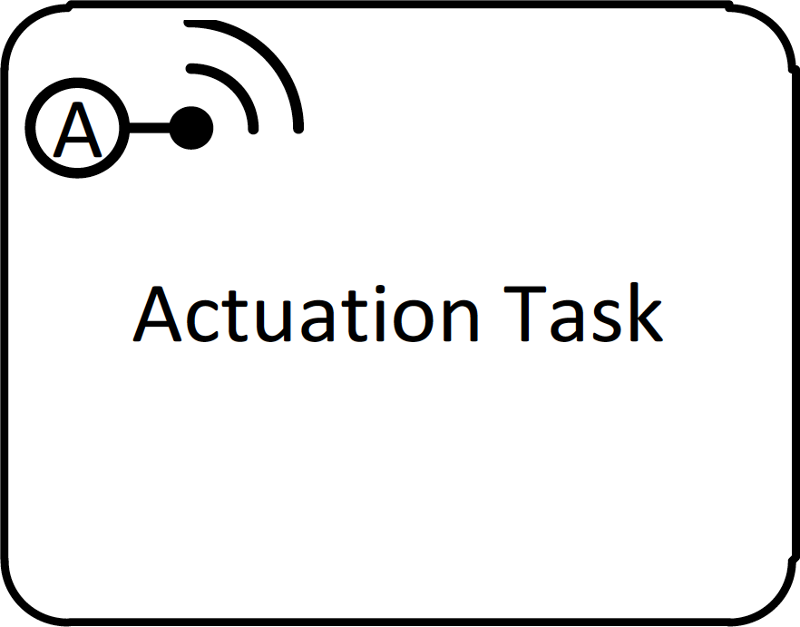
\includegraphics[height=2 cm,keepaspectratio,center]{figures/ActuationTask}
	\caption{Actuation Task \cite[S.44]{conceptsiotawarepm}}
	\label{fig:actuationtask}
\end{figure} 

\textbf{1.2. Sensing Activity}\\

Sensoren sind physische Elemente welche Bewegungen oder physikalische Werte erfasst und in elektronische Signale umwandelt. In der \ac{iot} Welt ist ein Sensor in der Lage den Zustand einer physischen Entität zu erfassen, dieses Erfassen des physischen Zustandes wird als sensing bezeichnet.\\
Sensoren sind in gewisser Weise als Gegenstück zu den Aktoren zu verstehen, ein Aktor ändert den Zustand einer physischen Entität während der Sensor seinen Zustand misst und somit die Änderung seines Zustandes registrieren kann. Als Gegenstück zu den Aktoren haben Sensing Activities keinen Daten Input aber dafür einen Daten Output. Allerdings werden auch diese weder weder durch die Business Process Execition Engine gestartet noch gemanaged sondern werden durch eine standardisierte Schnittstelle bereitgestellt und besitzen Anbindung an ein Data Object beziehungsweise Store \cite[S.45]{conceptsiotawarepm}. Der in Abbildung \ref{fig:sensingtask} ersichtliche Sachverhalt stellt den von der \ac{iapmc} entwickelten Sensing Task dar.

\begin{figure}[H]
	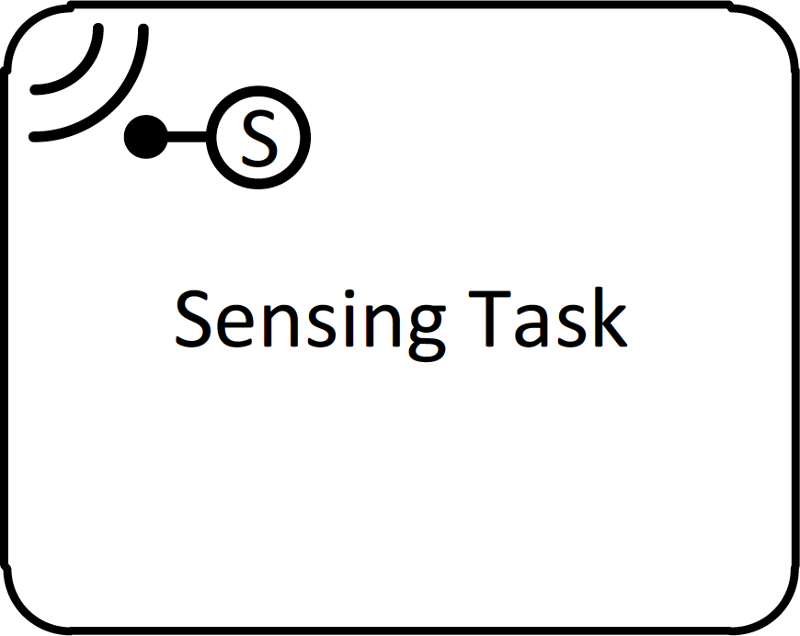
\includegraphics[height=2 cm,keepaspectratio,center]{figures/SensingTask}
	\caption{Sensing Task \cite[S.49]{conceptsiotawarepm}}
	\label{fig:sensingtask}
\end{figure} 

\textbf{2. IoT Device}\\

Wie in \ref{sec:DomainModel} beschrieben besitzt ein \ac{iot} Device die Fähigkeit den Status einer \ac{eoi} wahrzunehmen und mit einem Netzwerk zu kommunizieren. Des weiteren besitzt ein \ac{iot} Device im \ac{iota} Kontext die Möglichkeit aktiv den Status seiner physischen Entität oder einer anderen im \ac{iot} vorhandenen Netzwerk zu verändern. Mobiltelefone, ein Sensor-Knotenpunkt, einzelne Sensoren oder Aktuatoren sind Beispiele für ein \ac{iot} Device \cite[S.50]{conceptsiotawarepm}. Jeder Aktuator oder Sensor kann demnach als \ac{iot} Device angesehen werden. Hinzu kommt, dass \ac{iot} Devices Parameter besitzen welche die automatische Zuweisung durch die Auflösungsinfrastruktur anpassen und deren Verwendbarkeit bestimmen. \\
Wie in Abbildung \ref{fig:iotdevice} zu sehen ist das \ac{iot} Device, in diesem Fall ein Mobiltelefon, ein eigenständiger Akteur und besitzt eine eigene Swimlane. Durch das Aufklappen lassen sich die Parameter der Spezifikation anzeigen.

\begin{figure}[H]
	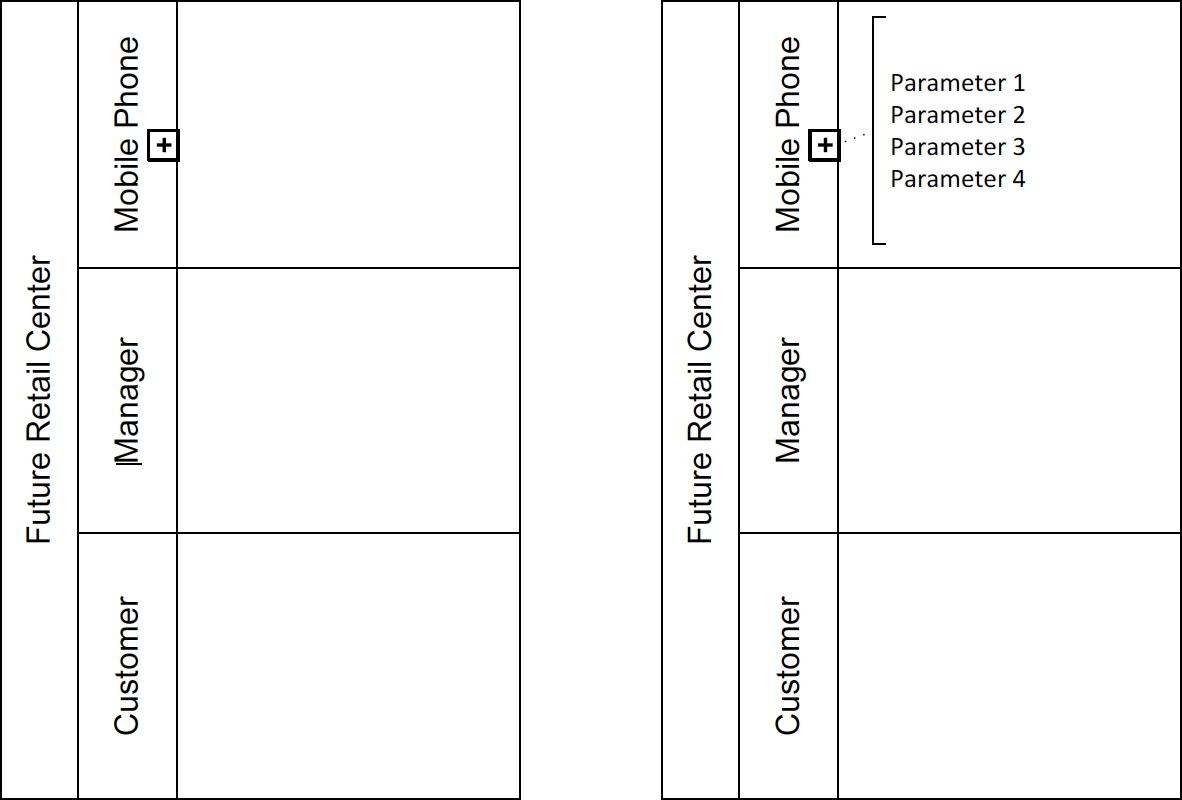
\includegraphics[height=7 cm,keepaspectratio,center]{figures/IoTDevice}
	\caption{IoT Device \cite[S.53]{conceptsiotawarepm}}
	\label{fig:iotdevice}
\end{figure} 

\textbf{3. Process Resources}\\

Die Definition von Ressourcen des \ac{iapmc} unterscheidet sich von der in \ref{sec:DomainModel} vorgestellten. Demnach seien Ressourcen in der Geschäftsprozessmodellierung ein abstraktes Konzept welches zur Klassifizierung der menschlichen oder technischen Einsatzfähigkeit während der Prozessauflösung für die Ausführung diene. So könne eine Ressource mehrere Aktivitäten ausführen und Aktivitäten könnten mehrere Ressourcen verwenden. Ein Beispiel für eine Ressource in der Prozessmodellierung ist ein IoT-Gerät wie ein Temperatursensor, der Messmöglichkeiten in Form von Prozessaktivitäten für die Prozessausführung bereitstellen kann\cite[S.54]{conceptsiotawarepm}. Eine Process Resource entspricht also einem Pool in \ac{bpmn} muss allerdings noch um Parameter für die Zuweisung sowie Metainformationen ergänzt werden.
\\

\textbf{4. Physical Entity}\\

Als Physical Entity also eine physische Entität wird ein Objekt aus der physischen Welt welches relevant für einen Benutzer oder eine Anwendung ist. Deshalb fällt in diesem Zusammenhang auch häufig der Begriff \acl{eoi} als ein Objekt an welchem Interesse besteht. Physische Instanzen in einem Prozess können für eine oder mehrere Aktivitäten relevant sein. Geschäftsprozesse gehen oft über Abteilungs- und Betriebsgrenzen hinweg, die sich in einem Prozess mit Hilfe von Pools und Lanes abbilden lassen. Physikalische Einheiten können innerhalb dieser Abteilungs- und Einsatzgrenzen existieren, aber auch darüber hinausgehen. Des weiteren können physische Entitäten für eine oder mehrere \ac{iot} Devices relevant sein\cite[S.58-59]{conceptsiotawarepm}. Physische Entitäten besitzen genauso wie \ac{iot} Devices Parameter die für die automatische Zuweisung von \ac{iot} Devices zu den physischen Entitäten relevant sind. Wie in Abbildung \ref{fig:physicalentity} zu sehen lassen sich Physical Entitys ebenso aufklappen um die Parameter anzeigen zu lassen wie die \ac{iot} Devices in Abbildung \ref{fig:iotdevice}. 

\begin{figure}[H]
	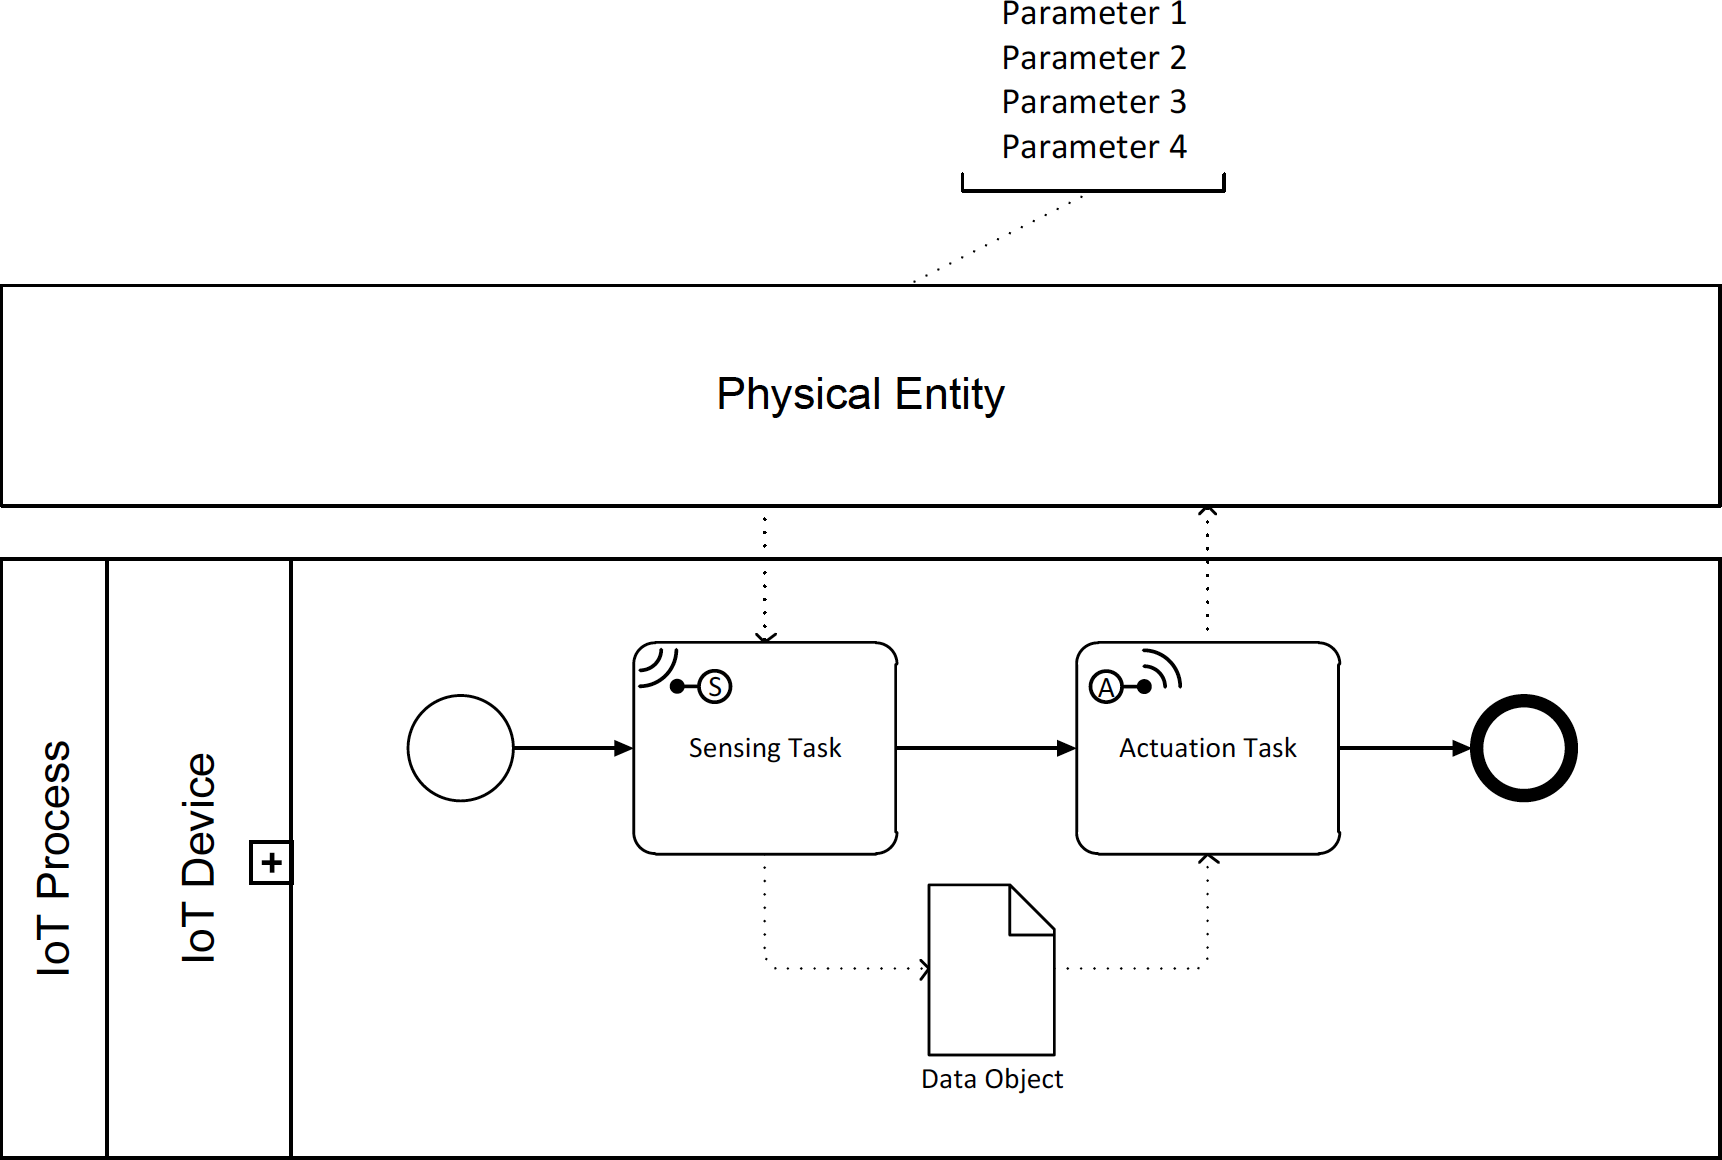
\includegraphics[height=7.3 cm,keepaspectratio,center]{figures/PhysicalEntity}
	\caption{Physical Entity \cite[S.62]{conceptsiotawarepm}}
	\label{fig:physicalentity}
\end{figure} 

\textbf{5. Real World Data Object / Store}\\

Ein Real-World Data Object stellt ein temporär gespeichertes Datenobjekt einer laufenden Prozessinstanz dar, das durch die Messung eines IoT Devices erzeugt wurde. Die Werte des Datenelements sind für andere Prozessbeteiligte sichtbar und existieren nicht über die Lebensdauer eines Prozesses hinaus. Das Real-World Data Object hat IoT-spezifische Eigenschaften, wie z.B. die unterschiedliche Qualität der Informationen. Neben einem Real-World Data Object kann ein Geschäftsprozess auch einen Real-World Data Store enthalten. Im Gegensatz zum Real-World Data Object stellt der Real-World Data Store persistente Daten dar und existiert über die Lebensdauer einer Prozessinstanz hinaus. Der Real-World Data Store kann von den Teilnehmern des Prozesses sowie von Teilnehmern außerhalb des Prozesses abgefragt oder aktualisiert werden. Real-World Data Objects sowie Real-World Data Stores besitzen Eigenschaften welche darüber Auskunft erteilen wann welches \ac{iot} Device den Datensatz über welche Physische Entität erstellt hat \cite[S.64-65]{conceptsiotawarepm}. In Abbildung \ref{fig:datastore} und \ref{fig:datastore} sind die Modelle mehrerer Data Objects beziehungsweise Data Stores mit ausgeklappten Eigenschaften zu sehen.

\begin{figure}[H]
	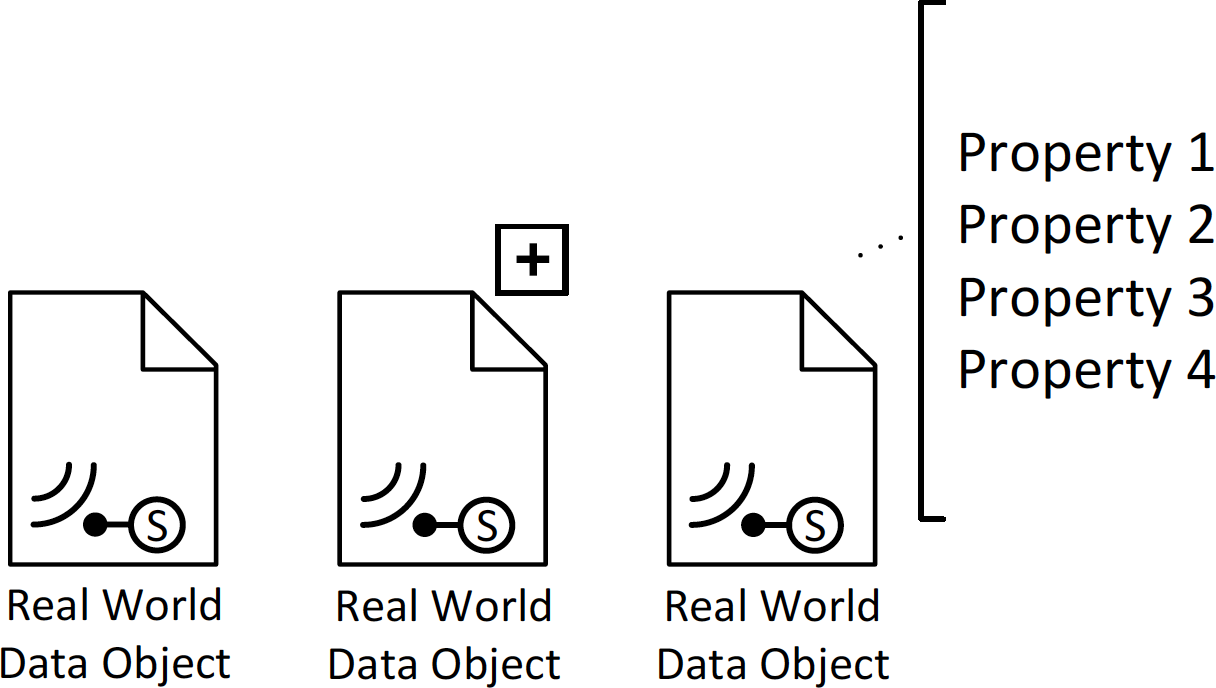
\includegraphics[height=3.5 cm,keepaspectratio,center]{figures/DataObject}
	\caption{Data Object \cite[S.67]{conceptsiotawarepm}}
	\label{fig:dataobject}
\end{figure} 

\begin{figure}[H]
	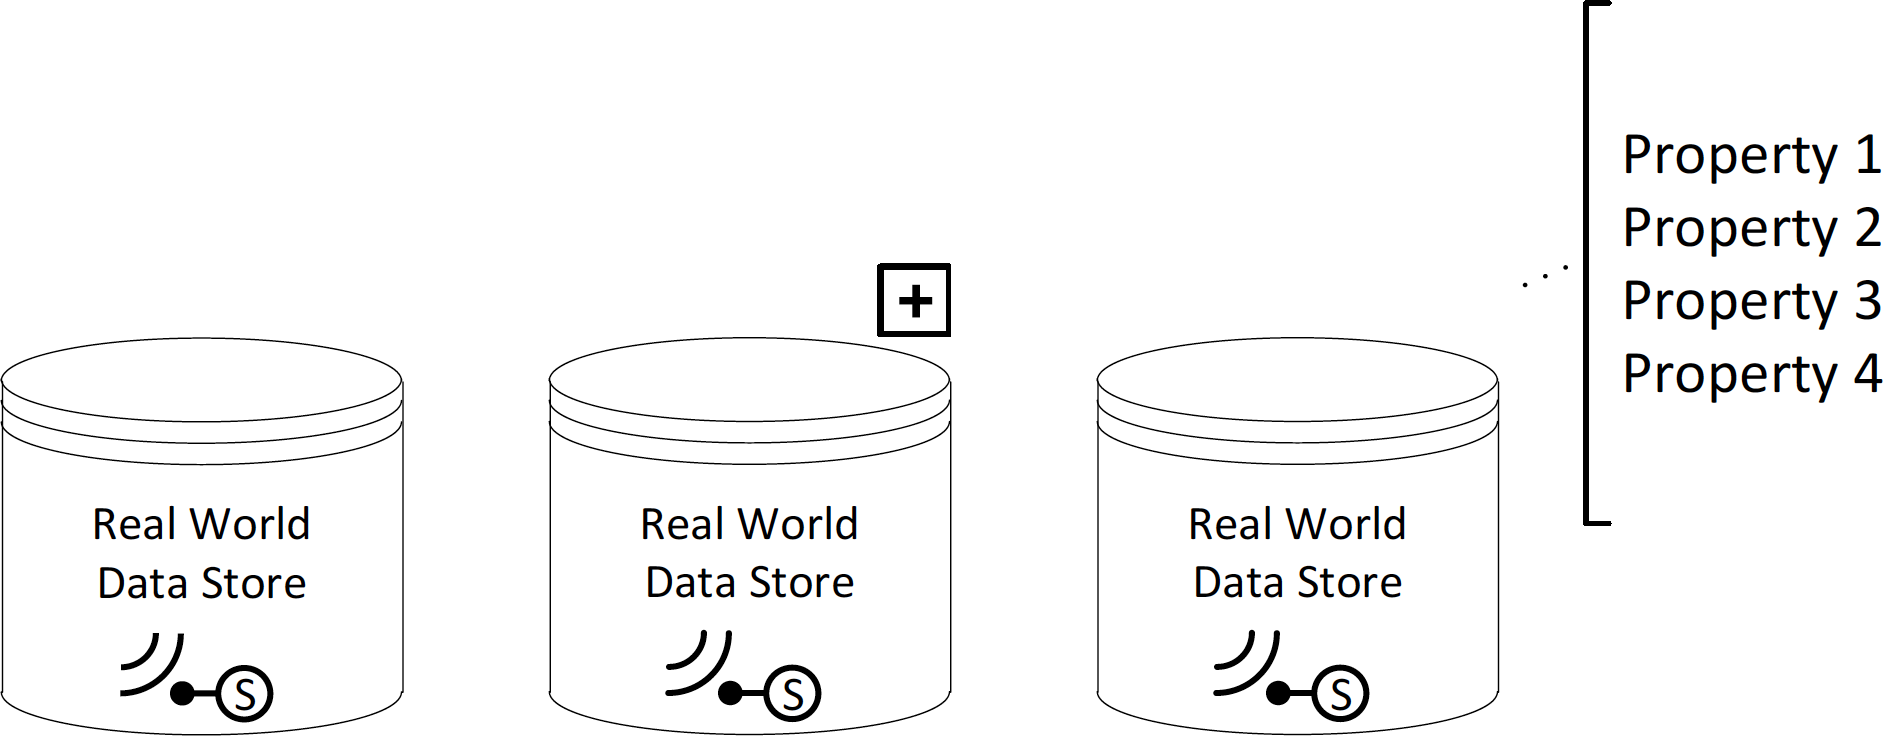
\includegraphics[height=3 cm,keepaspectratio,center]{figures/DataStore}
	\caption{Data Store \cite[S.67]{conceptsiotawarepm}}
	\label{fig:datastore}
\end{figure} 

\textbf{6. Mobility Aspect}
\newline
Mobilität kann Prozessbeteiligte wie IoT Devices oder die Physical Entitys betreffen, welche dadurch die Aktivitäten beeinflussen, für die sie verantwortlich sind. Dieser Aspekt bezieht sich sowohl auf IoT-Aktivitäten als auch auf normale Aktivitäten. In Folge dessen werden Prozesse oder Teilprozesse durch das mobile Verhalten ihrer "Teilnehmer", also deren Ortswechsel beeinflusst. So können Prozesse aufgrund von dem Erreichen eines \ac{eoi} an einem bestimmten Ort oder der signifikanten Lageänderung ausgelöst werden beziehungsweise Abhängig davon sein. Deshalb benötige \ac{bpmn} Erweiterungen um zu Kennzeichnen wenn ein Prozess, ein Prozessteilnehmer, eine Prozessentscheidung oder eine Aktivität mobil seien \cite[S.68-70]{conceptsiotawarepm}. Das in Abbildung \ref{fig:mobile} auf der linken Seite zu sehende Symbol indiziert, dass die Komponente in welcher sie verwendet wird mobil ist während das rechte Symbol die Ortsabhängigkeit darstellt.

\begin{figure}[H]
	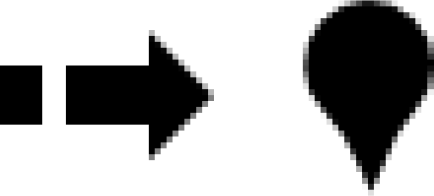
\includegraphics[height=0.75 cm,keepaspectratio,center]{figures/Mobile}
	\caption{Mobile Property, Location based Property\cite[S.71]{conceptsiotawarepm}}
	\label{fig:mobile}
\end{figure} 

Zusammengefasst lässt sich das \ac{iota} Modellierungskonzept an dem in Abbildung \ref{fig:iotaprocess} veranschaulichen. Hierbei geht es um einen Sensor basierten Qualitätskontrollprozess. Eine Orchidee ist hierbei die Physische Entität welche mittels eines smarten Temperatur Sensors überwacht wird. Alle 60 Sekunden wird ein sensing Task ausgelöst welcher die Temperatur der Orchidee misst und das daraus resultierende Data Object an ein Backend System weiterleitet. Sofern die Temperatur nicht außerhalb der Norm liegt endet der Prozess. Ansonsten wird sowohl eine Alarm Benachrichtigung auf dem SmartPhone Ted angezeigt, welcher ein mobiler Prozessteilnehmer ist, sowie eine Berechnung des neuen Preises des Backend Systems veranlasst. Der angepasste Preis wird an einen Aktuator, das Regaletikett weitergeleitet, welcher den neuen Preis der Orchidee anpasst und somit den Prozess beendet. In diesem Prozess werden ein Großteil des \ac{iapmc} sinnvoll dargestellt und eingesetzt.

\begin{figure}[H]
	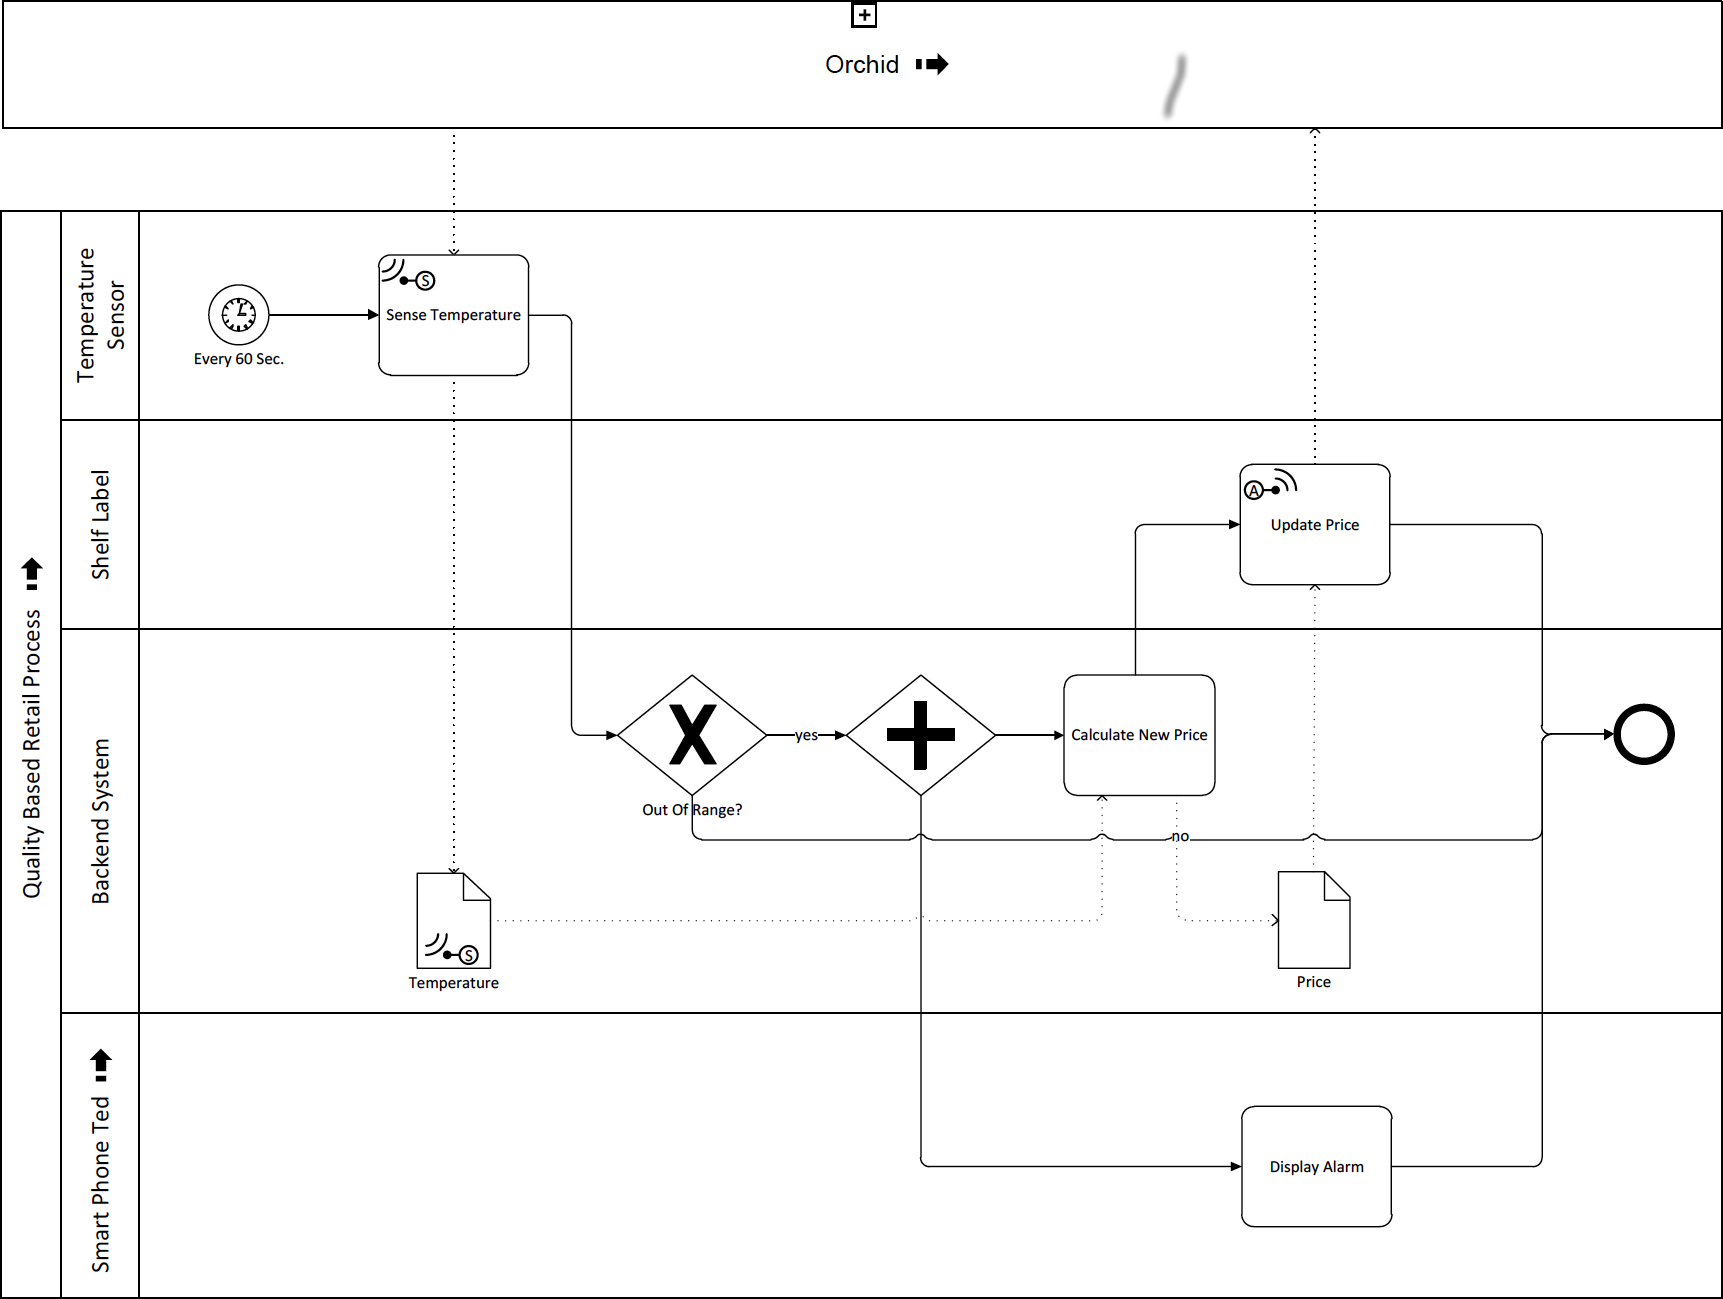
\includegraphics[height=11 cm,keepaspectratio,center]{figures/iotaprocess}
	\caption{\ac{iapmc} Beispiel\cite[S.81]{conceptsiotawarepm}}
	\label{fig:iotaprocess}
\end{figure} 

\textbf{Bewertung}

\begin{filecontents}{\jobname-iotabewertung.tex}
	\begin{longtable}{P{4cm}|X}
		\caption{Umsetzung der IoT spezifischen Anforderungen durch das IoT-A Modellierungskonzept}\\
		\label{table:evaluierungskriterien}
		% Definition des ersten Tabellenkopfes auf der ersten Seite
		\textbf{Anforderung} & \textbf{Erklärung}   \\ \hline
		\endfirsthead % Erster Kopf zu Ende
		%  Definition des Tabellenkopfes auf den folgenden Seiten
		\textbf{Anforderung} & \textbf{Erklärung}  \\ \hline
		\endhead
		% Ab hier kommt der Inhalt der Tabelle
		Device als Akteur & Im \ac{iota}Modellierungskonzept wird \ac{bpmn} um die Rolle eine IoT Devices erweitert, dieser besitzt Parameter welche die Zuweisung von Devices zu \ac{eoi} ermöglicht.\\ \hline
		Physische Dinge  & Genauso wie Devices besitzen \ac{eoi} im \ac{iota} Konzept Parameter welche die Zuweisung zu Device und generierten Informationen ermöglicht.\\ \hline
		Spezielle Aufgabentypen & Mit der Einführung von Actuation Task und Sensing Task werden die grundlegendsten Funktionsweisen von \ac{iot} Devices abgedeckt.\\ \hline
		Informationen  & Die von den \ac{iot} Devices bereitgestellten Informationen werden durch eine Erweiterung von der vorhanden DataObjects in \ac{bpmn} umgesetzt. Diese besitzen Metadaten über ihre Herkunft, Erstellungsort und Zeit sowie ihrer Qualität.\\ \hline
		Mobiltät & Prozessteilnehmer und Aufgaben können durch die Einführung der Mobile Property beziehungsweise Location-based Activity als mobil gekennzeichnet werden. Allerdings handelt es sich hierbei eher um eine kosmetische Erweiterung als um eine funktionale. Eine ortsabhängige Ausführung von Task wird durch die Erweiterung nicht gewährleistet.\\ \hline
		Granularität & Durch die klassische \ac{bpmn} Elemente lassen sich Prozesse aus beliebig vielen geringer komplexen Subprocesses zusammenstellen.\\ 
	\end{longtable}
\end{filecontents}
\LTXtable{\textwidth}{\jobname-iotabewertung.tex}

\subsubsection{BPMN4CPS}
\ac{bpmn4cps} stellt ähnlich wie \ac{iapmc} ein Konzept vor welches die \ac{bpmn} um Besonderheiten von \ac{iot} beziehungsweise \ac{cps} erweitern soll. Dieses Konzept wurde erstmalig bei der 25 IEEE Conference on Enabling Technologies: Infrastructure for Collaborative Enterprises vorgestellt. Ziel hierbei ist es den Entwicklern zu ermöglichen, CPS-Elemente, -Konzepte und -Eigenschaften bei der Modellierung von CPS-Prozessen präzise und effizient zu berücksichtigen. Hierfür wurden Relevante Eigenschaften von \ac{cps} herausgearbeitet auf welche im folgenden Abschnitt eingegangen wird.
Die für \ac{cps} relevanten Charakteristiken lauten nach \cite{BMPN4CPS} wie folgt:\\

\textbf{Aufgaben Typen}\\
Im physischen Prozess können CPS-Aufgaben eine physische oder eine manuelle Aufgabe sein. Die physische Aktivität liefert Sensordaten oder führt Aktionen aus, die sich auf die physische Welt auswirken. Sie können die Aktivität eines Sensors wie der Temperaturmesssensor oder die Aktivität eines Aktors wie die Luftkühlung durch eine Klimaanlage sein. Während eine manuelle Aufgabe von einem Menschen ohne die Hilfe eines Geräts oder einer Anwendung ausgeführt werden soll.\\

\textbf{Eintäten-/Resourcen basiertes Konzept}\\
Das physikalische Gerät hat eine schlechte Rechenleistung und einen dynamischen Zustand. Die Ausführung einer physischen Aktivität kann sich auf die physischen Einheiten und das Gerät auswirken, indem sie ihre lokalen Zustände ändert. Daher müssen während der Modellierungsphase weitere Informationen über die beteiligte Entität, Ressource oder das Device bereitgestellt werden\\

\textbf{Event basierte, Befehl/Aktions basierte und periodische Aufgaben}\\
Eine Aufgabe kann durch ein Ereignis oder eine Befehlsnachricht ausgelöst werden. Es kann auch eine periodische Aufgabe sein, die in jedem Intervall oder zu jedem Zeitpunkt stattfinden soll. Diese Annotationen werden von BPMN unterstützt.\\

\textbf{Mobilität}\\
Das physische Gerät kann mobil oder statisch sein. Diese Eigenschaft ist wichtig, da zusätzliche Informationen beim mobilen Verhalten zur Laufzeit berücksichtigt werden müssen.\\

\textbf{Verfügbarkeit}\\
Eine physische Aktivität kann nur dann einsatzbereit sein, wenn ihr Anbieter zeitlich und räumlich verfügbar ist.\\

\textbf{Zeitliche Anforderungen}\\
Das zeitliche Verhalten ist die zentrale Eigenschaft der physikalischen Prozesse, bei denen die Zeit entscheidend ist. Besonders bei kritischen Anwendungen müssen physikalische Maßnahmen zur richtigen Zeit und zum richtigen Zeitpunkt getroffen werden\\

\textbf{Räumliche Eigenschaften}\\
Sind die Anforderungen, welche mit physischen Aktivitäten verbunden sind. Sie stellen den Ort dar, an dem die Aktivität ausgeführt werden soll und den betroffenen Bereich, der durch die Aktivität des Sensors beziehungsweise des Aktors beeinflusst werden soll.\\

\textbf{Zeit Räumliche Eigenschaften}\\
Die physische Umgebung ist kontinuierlich dynamisch. Diese Dynamik kann raum-zeitlicher Natur sein, die Zeit- und Rauminformationen kombiniert. Zum Beispiel ändert sich der Zustand eines physischen Objekts kontinuierlich entsprechend seiner Position in Raum und Zeit.\\

\textbf{Kontext Eigenschaften}\\
Der Kontext und die reale Umgebung, in der die physischen Aktivitäten ausgeführt werden, beeinflussen ihr Verhalten. So besteht beispielsweise ein enger Zusammenhang mit der physischen Bewegung eines Fahrzeugs und seiner Umgebung\\

\textbf{BPMN4CPS Modellierungskonzept}\\

\textbf{1. Aufgabentypen}\\
Für die Umsetzung eines Cyber Physischen Prozesses sind laut des \ac{bpmn4cps} mindestens drei Pools nötig. Der erste Pool stellt den physischen Prozess dar, der zweite Pool den Cyber Prozess und der dritte einen Controller welcher für die Kommunikation zwischen dem Cyber Prozess und dem phyischen Prozess orchestriert. Außerdem wurde der in Abbildung \ref{fig:physicaltask} sichtbaren Physical Task  angelegt. Dieser unterscheidet zwischen einem Actuator's Task und einem Sensor's Task. Ein Actuator's Task nimmt Einfluss auf den Zustand einer physical Entity während ein Sensor's Task dessen Zustand misst.

\begin{figure}[H]
	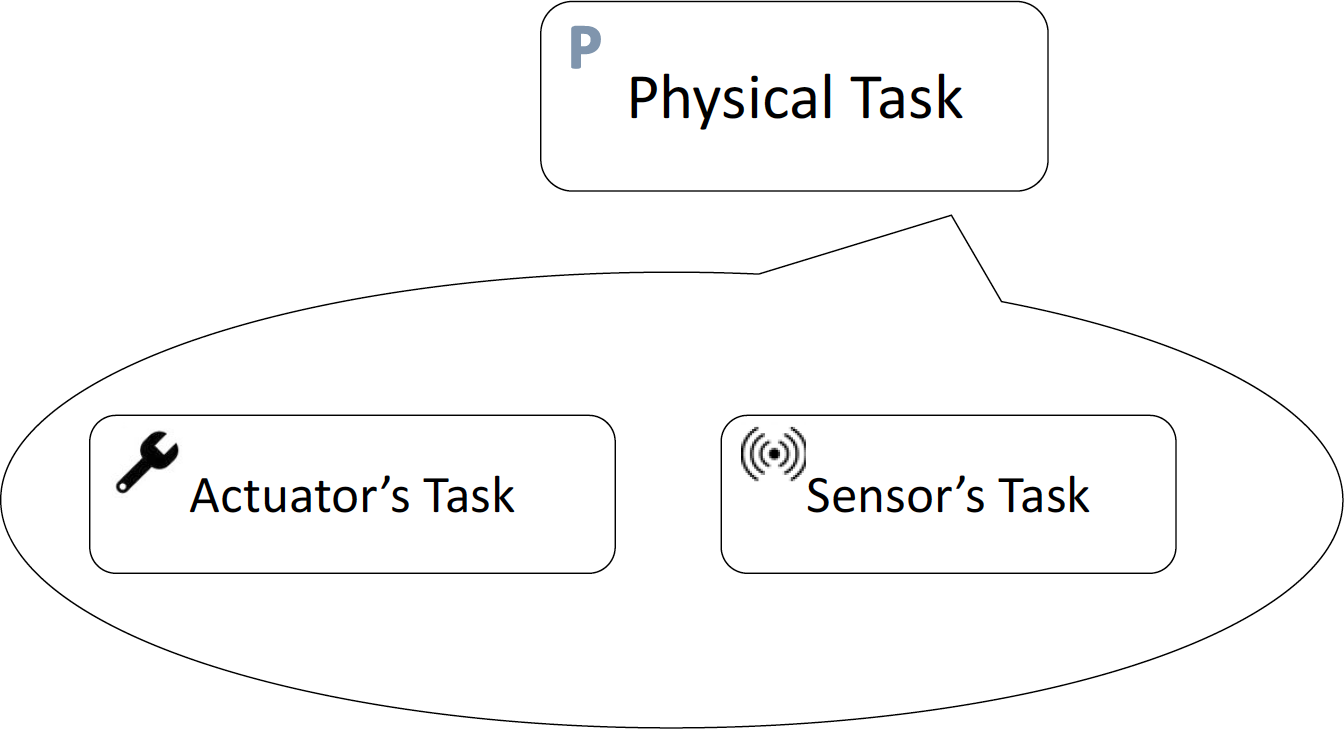
\includegraphics[height=4 cm,keepaspectratio,center]{figures/PhysicalTask}
	\caption{Physical Task\cite{BMPN4CPS}}
	\label{fig:physicaltask}
\end{figure} 

Des weiteren wurde der in Abbildung \ref{fig:cybertask} zu sehende Cyber Task angelegt welcher eine Erweiterung des schon in \ac{bpmn} bestehenden Service Task darstellt. Dieser Task besitzt drei Ausführungen den Embedded Service Task, welcher einen Cyber Task darstellt der an einem \ac{iot} Device selbst ausgeführt wird, den Web Serice Task, bei dem die Aufgabe an einen Webservice weitergeleitet wird und den Cloud Service Task welcher von einem Cloud Service ausgeführt wird.

\begin{figure}[H]
	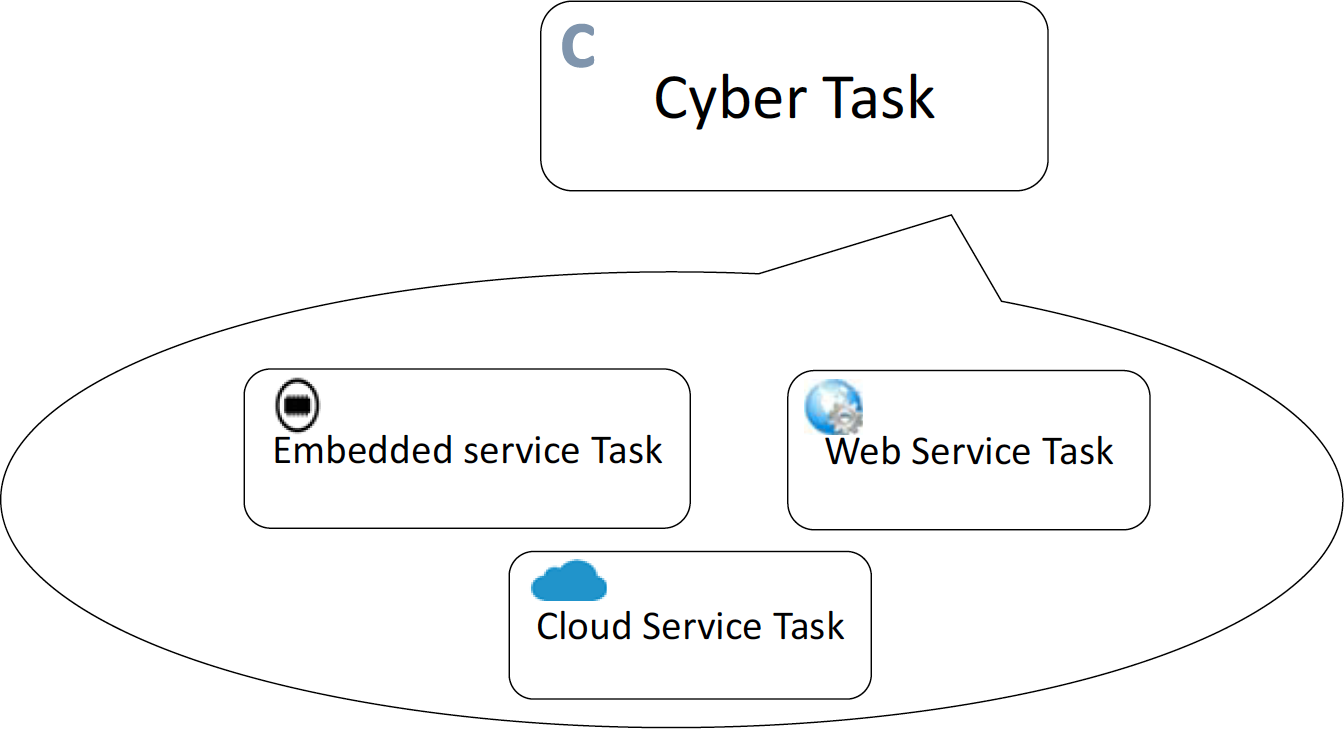
\includegraphics[height=4 cm,keepaspectratio,center]{figures/CyberTask}
	\caption{Physical Task\cite{BMPN4CPS}}
	\label{fig:cybertask}
\end{figure} 


In der Abbildung \ref{fig:bpmn4cpsProcess} ist ein minimaler Beispielprozess des \ac{bpmn4cps} zu sehen. Wie beschrieben sind die drei Standard Pools eines \ac{cps} zu sehen. Im physischen Prozess wird der gemessene Zustand einer pyhsischen Entität dem Controller mitgeteilt. Dieser leitet ihn an den Cyber Prozess weiter und führt selbst einen Embedded Service Task aus. Der Cyber Prozess führt zunächst einen Cloud Service Task aus und danach parallel einen Webservice Task sowie eine Cyber Activity, danach werden die Ergebnisse wieder dem Controller gesendet. Dieser wandelt sie in einen Befehl um welcher auf dem Physischen Prozess durch einen Actuator's activity ausgeführt wird, welche den Zustand einer physischen Entität ändert. 

\begin{figure}[H]
	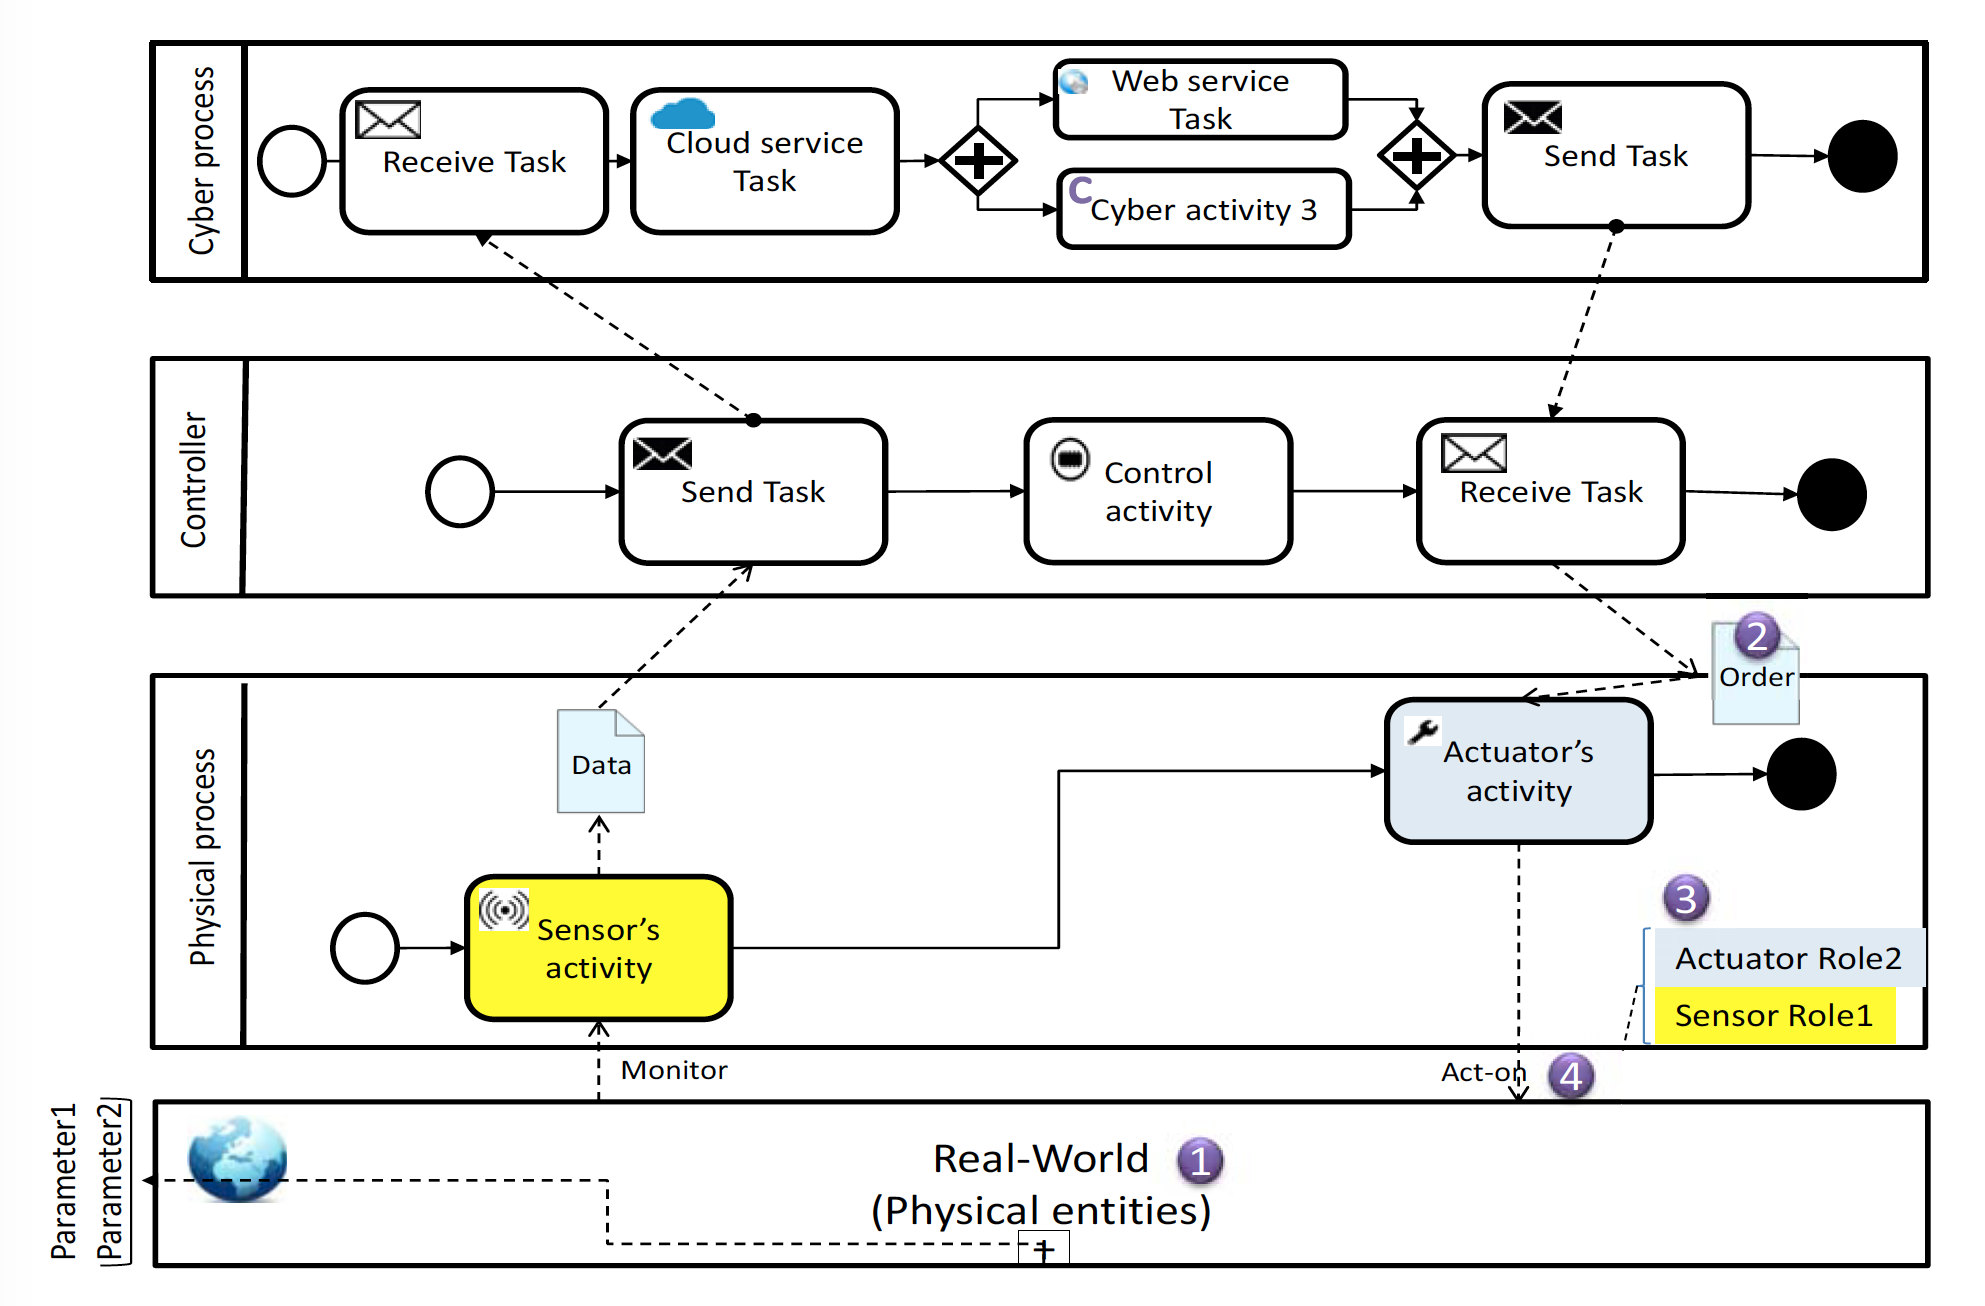
\includegraphics[height=10cm,keepaspectratio,center]{figures/bpmn4cpsProcess}
	\caption{Beispielprozess nach \ac{bpmn4cps} \cite{BMPN4CPS}}
	\label{fig:bpmn4cpsProcess}
\end{figure} 

\textbf{Bewertung}

\begin{filecontents}{\jobname-bpmn4cpsbewertung.tex}
	\begin{longtable}{P{4cm}|X}
		\caption{Umsetzung der IoT spezifischen Anforderungen durch das BPMN4CPS Modellierungskonzept}\\
		\label{table:evaluierungskriterien}
		% Definition des ersten Tabellenkopfes auf der ersten Seite
		\textbf{Anforderung} & \textbf{Erklärung}   \\ \hline
		\endfirsthead % Erster Kopf zu Ende
		%  Definition des Tabellenkopfes auf den folgenden Seiten
		\textbf{Anforderung} & \textbf{Erklärung}  \\ \hline
		\endhead % Zweiter Kopf ist zu Ende
		% Ab hier kommt der Inhalt der Tabelle
		Device als Akteur & In \ac{bpmn4cps} werden Devices nicht als eigene Lane dargestellt, da dies aber bei einer großen Anzahl an Lanes führen würde sondern wird über eine farbliche Zuweisung dargestellt. Devices lassen sich über Parameter eindeutig physischen Dingen zuweisen. \\ \hline
		Physische Dinge  & Die \ac{bpmn4cps} spezifischen Aufgabentypen beziehen sich direkt auf die physischen Dinge und überwachen beziehungsweise verändern dessen Zustand. Die physische Entität selbst wird als Prozess Teilnehmer dargestellt und ist mit dem physischen Prozess Pool verbunden.\\ \hline
		Spezielle Aufgabentypen & \ac{bpmn4cps} Konzept bietet zum einen Physical Tasks welche in Actuators Task und Sensing Task unterschieden wird und zum Anderen Cyber Tasks die sich in WebServiceTasks beziehungsweise CloudServiceTasks sowie EmbeddedService Tasks unterscheiden.\\ \hline
		Informationen  & Das \ac{bpmn4cps} Konzept verwendet für die von Devices erzeugten Informationen lediglich die standard \ac{bpmn} Elemente.\\ \hline
		Mobiltät & Devices können über den Parameter isMovable als mobil gekennzeichnet werden, besitzen allerdings keinen optischen Indikator dafür. Tasks sind besitzen weder Parameter über die Mobilität noch lassen sich diese ortsabhängig ausführen.\\ \hline
		Granularität & Durch die klassische \ac{bpmn} Elemente lassen sich Prozesse aus beliebig vielen geringer komplexen Subprocesses zusammenstellen.\\
	\end{longtable}
\end{filecontents}
\LTXtable{\textwidth}{\jobname-bpmn4cpsbewertung.tex}

\subsection{UML Aktivitätsdiagramm basierte Ansätze}
Eine Grundlegende Beschreibung zu \ac{uml} ist in Kapitel \ref{uml} zu finden. Deshalb wird in diesem Unterkapitel \ac{bpmn} lediglich auf die Verwendbarkeit für die Modellierung von \ac{iot} Workflows bewertet.
\textbf{Bewertung}. Trotz ausgiebiger Recherche konnten keine \ac{iot} spezifischen Erweiterung für \ac{uml} Aktivitätdiagramme gefunden werden. Deshalb wird in diesem Kapitel lediglich das Standard \ac{uml} Aktivitätsdiagramm bewertet.

\begin{filecontents}{\jobname-umlbewertung.tex}
	\begin{longtable}{P{4cm}|X}
		\caption{Umsetzung der IoT spezifischen Anforderungen durch UML Aktivitätsdiagramme}\\
		\label{table:evaluierungskriterien}
		% Definition des ersten Tabellenkopfes auf der ersten Seite
		\textbf{Anforderung} & \textbf{Erklärung}   \\ \hline
		\endfirsthead % Erster Kopf zu Ende
		%  Definition des Tabellenkopfes auf den folgenden Seiten
		\textbf{Anforderung} & \textbf{Erklärung}  \\ \hline
		\endhead % Zweiter Kopf ist zu Ende
		% Ab hier kommt der Inhalt der Tabelle
		Device als Akteur & In \ac{uml} Aktivitätsdiagrammen lassen sich Devices als Swimlanes darstellen und bieten somit eine Gruppierung von Knoten also Aufgaben, welche vom Device übernommen werden.\\ \hline
		Physische Dinge  & Physische Dinge können in Aktivitätsdiagrammen als Objektknoten dargestellt werden deren Zustand durch Aktionsknoten verändert wird. Eine Darstellung als eigene Lane wie es in \ac{bpmn} existiert ist nicht möglich da hier keine zugeklappte Lane existiert und das Physische Objekt an sich keine eigenen Aufgaben übernimmt.\\ \hline
		Spezielle Aufgabentypen & \ac{uml} Aktivitätsdiagramme besitzen keine besondere Form von Aufgaben sondern besitzen lediglich eine Darstellung durch Aktionsknoten. \\ \hline
		Informationen  & Informationen werden klassischer Weise als Objektknoten modelliert, diese können beliebig viele Attribute enthalten. Eine Modellierung von Informationen mit dem selben graphischen Element wie das physische Ding würde das Modell jedoch \\ \hline
		Mobiltät & UML Aktivitätsdiagramme bieten keine Weise die Mobilität von Prozessteilnehmern oder die Ortsabhängigkeit von Aktionen darzustellen.\\ \hline
		Granularität & Prozesse könne aus mehreren Unterprozessen zusammengesetzt werden.\\
	\end{longtable}
\end{filecontents}
\LTXtable{\textwidth}{\jobname-umlbewertung.tex}

\subsection{Geschäftsregel basierte Ansätze}
Da im Kapitel \ref{businessrules} schon darauf eingeganen wurde, dass sich der \ac{ecaa} Ansatz nur für die Darstellung von sehr kurzen Prozessen eignet, wird hier die Verwendbarkeit von \ac{eepk} für die Modellierung von \ac{iot} Geschäftsprozessen geprüft. Eine ausgiebige Recherche brachte keine Ergebnisse über Erweiterungen von \ac{eepk} im Bezug auf IoT Modellierung, weshalb in diesem Kapitel lediglich die Standard \ac{eepk} auf die Eignung zur Darstellung von \ac{iot} Workflows bewertet wird.
\textbf{Bewertung}

\begin{filecontents}{\jobname-businessrulesbewertung.tex}
	\begin{longtable}{P{4cm}|X}
		\caption{Umsetzung der IoT spezifischen Anforderungen durch eEPK}\\
		\label{table:evaluierungskriterien}
		% Definition des ersten Tabellenkopfes auf der ersten Seite
		\textbf{Anforderung} & \textbf{Erklärung}   \\ \hline
		\endfirsthead % Erster Kopf zu Ende
		%  Definition des Tabellenkopfes auf den folgenden Seiten
		\textbf{Anforderung} & \textbf{Erklärung}  \\ \hline
		\endhead % Zweiter Kopf ist zu Ende
		
		% Ab hier kommt der Inhalt der Tabelle
		Device als Akteur & Device kann als Stelle der Zuständigkeit darstellen lassen. \\ \hline		
		Physische Dinge  & Physisches Ding kann sich als Informationsquelle in \ac{eepk} darstellen lassen allerings kann der Zustand von Informationsquellen nicht verändert werden.\\ \hline	
		Spezielle Aufgabentypen & \ac{eepk} besitzt für die Darstellung von Aufgaben nur das Modell der Funktion.\\ \hline		
		Informationen  & Informationen besitzen ihr eigenes Symbol in \ac{eepk} allerdings wird dieses bereits für die Modellierung des physischen Dings verwendet was zu Komplikationen bei der Interpretation des Modells führen kann. Des Weiteren lassen sich die \ac{iot} spezifischen Anforderungen an die Informationen nicht darstellen.\\ \hline		
		Mobiltät & In \ac{eepk} Durch das Eintreten bestimmter Ereignisse lässt sich die Ortsabhängigkeit von Aufgaben abbilden. Die Mobilität von den \ac{eoi} selbst lässt sich allerdings nicht darstellen.\\ \hline
		Granularität & Eine Aufteilung eines Prozesses in mehrere Unterprozesse ist nicht möglich.\\
	\end{longtable}
\end{filecontents}
\LTXtable{\textwidth}{\jobname-businessrulesbewertung.tex}

\subsection{Auswahl eines Modellierungskonzepte}\label{auswahl}
Für die Bewertung und Auswahl eines geeigneten Modellierungskonzeptes werden die in \ref{anforderungen} definierten \ac{iot} spezifischen Anforderungen verwendet. Dieses Unterkapitel dient lediglich als Gegenüberstellung der einzelnen Modellierungskonzepte.  Die ausführliche Bewertung ist in den jeweiligen Kapiteln der Modellierungskonzepte zu finden. 

%Security ist für die Prozesse wichtig, muss aber in den darunterliegenden Schichten Anwendungsarhcitektur, Informationsarchiektur und Technologische Archiektur umgesetzt werden. Also von der Software die diese Prozesse ausführt.

\begin{filecontents}{\jobname-Evaluierung.tex}
	\begin{longtable}{| l |c|c|c|c|c|c|}
		\caption{Bewertung der Modellierungsmethoden}\\ \hline
		\label{table:Evaluierung}
		% Definition des ersten Tabellenkopfes auf der ersten Seite
		 & \textbf{IoT - A} & \textbf{BPMN4CPS} & \textbf{PD}\footnotemark[1] & \textbf{CD}\footnotemark[2] & \textbf{AD}\footnotemark[3] &\textbf{eEPK}  \\\hline
		\endfirsthead % Erster Kopf zu Ende
		
		%  Definition des Tabellenkopfes auf den folgenden Seiten
		& \textbf{IoT - A} & \textbf{BPMN4CPS} & \textbf{PD}\footnotemark[1] & \textbf{CD}\footnotemark[2] & \textbf{AD}\footnotemark[3] &\textbf{eEPK} \\ \hline		
		\endhead % Zweiter Kopf ist zu Ende
		\multicolumn{7}{P{10.8cm}}{\textit{+ = Anforderung erfüllt, 0 = Anforderung teilweise erfüllt, - = Anforderung nicht erfüllt}}\\
		\endlastfoot


		% Ab hier kommt der Inhalt der Tabelle
		Device als Akteur & +  & + & 0 & 0 & 0 & 0 \\ \hline
		
		Physische Dinge  & + & + & 0 & 0 & 0 & - \\ \hline

		Spezielle Aufgabentypen & + & + & - & - & -& - \\ \hline

		Informationen  & + & - & - & - & - & - \\ \hline

		Mobilität & 0 & - & - & - & - & 0 \\ \hline

		Granularität & + & + & + & + & + & - \\ \hline

	\end{longtable}
\end{filecontents}
\LTXtable{\textwidth}{\jobname-Evaluierung.tex}

Wie sich der Tabelle entnehmen lässt erfüllt das \ac{iota} Modellierungskonzept nahezu alle \ac{iot} spezifischen Anforderung an die Modellierung und wird deshalb in Kapitel \ref{usecasemodellierung} für die Modellierung des Anwendungsfalles verwendet.

\footnotetext[1]{PD = BPMN Prozessdiagramm}
\footnotetext[2]{CD = BPMN Choreographiediagramm}
\footnotetext[3]{AD = UML Aktivitätsdiagramm}

\newpage

\section{Anwendung des Konzeptes} \label{anwendung}
%http://www.bpm-guide.de/2015/04/09/orchestration-using-bpmn-and-microservices/
%Anforderung und bestehende Systeme bestimmen Modellierung
Die Herangehensweise für die Modellierung von \ac{iot} Workflows ist stark von den verwendeten Devices sowie von den funktionalen und nicht funktionalen Anforderungen abhängig. Wenn die lokale Auswertung der Daten auf den Geräten aufgrund der vorhandenen Rechenleistung nicht möglich ist, so müssen die Daten einem zentralen Service übermittelt werden der die benötigte Rechenleistung besitzt.\\
Wenn alle Services gebündelt durch ein Backend bereitgestellt werden, so wird die Kommunikation der Prozessteilnehmer zwangsläufig durch das Backend orchestriert (Hub and Spoke).\\
Sinnvoll ist es jedoch wenn \ac{iot} Devices die in einem Zusammenhang zu einander stehen zu Multi Device Gateways  gebündelt werden und sich somit im Modell als Pool darstellen lassen, was die Übersichtlichkeit des Modells verbessert. Dadurch wird zum einen eine Bottom Up Herangehensweise der Modellierung möglich zum anderen kann eine Art Microservice Architektur erreicht werden.\\
Gateways können entweder mit ausreichend Rechenleistung ausgestattet werden um die Daten selbst zu bearbeiten oder aufgrund der vom Backend ausgewerteten Daten Entscheidungen zu fällen und selbstständig mit den anderen Multi Device Gateways zu kommunizieren(Peer to Peer).\\

Für die Umsetzung des Prozesses in einen Workflow gibt es für beide Vorgehensweise Vor- und Nachteile, lose gekoppelte peer-to-peer Choreographie erlauben eine einfache Anpassung an sich schnell ändernde Geschäftsbedingungen während eine Orchestrierung eine einfache Überwachung des Prozessablaufes ermöglicht\cite{orchVSchoreo}. Eine Orchestrierung von Microservices widerspricht in der heutigen Zeit jedoch nicht mehr dem Konzept des \ac{bpm} sondern wird von  immer mehr \ac{bpm} Engines wie zum Beispiel Camunda\cite{camundamicroservices}, zeebe\cite{zeebeio} und Netflix Conductor\cite{conductor} unterstützt.\\
Bern Rücker Mitbegründer der Camunda Workflow Engine sieht hierbei jedoch keine entweder oder Frage sondern stellt in seinem Blog eine Kombination aus Choreographie und Orchestrierung vor bei dem die Orchestrierung lokal in den eizelnen Microservices stattfindet während der Gesamtprozess als Choreographie implementiert wird bei dem lediglich Nachrichten untereinander ausgetauscht werden\cite{orchandchoreo}. Hierbei könnte jeder Microprocess eine eigene Process Engine besitzen \cite{bpmmonolith}.\\

\subsection{Fallbeispiel}
Wie in Kapitel \ref{motivation} beschrieben ist bietet \ac{iot} neben der Optimierung von bestehenden Geschäftsprozessen auch die Möglichkeit der Gestaltung völlig neuer Geschäftsmodelle. Ein Beispiel für eine Generierung neuer Geschäftsmodelle stellt ein durch \ac{iot} ermöglichter fahrstilabhängiger Versicherungstarif dar.\\
Heutige Versicherungstarife setzen sich aus einer Vielzahl an statistischen Kennzahlen zusammen welche nur bedingt vom Versicherungsnehmer beeinflusst werden können. Diese Kalkulation kommt in den meisten Fällen aggressiven Fahrern zu Gute und geht zu Lasten von vorsichtigen Fahrern. Moderne Kraftfahrzeuge sind mit einer Vielzahl an Sensoren und der Möglichkeit der Kommunikation ausgestattet und entsprechen somit den in Tabelle \ref{table:smartObjectsCharacteristics} vorgestellten Charakteristiken smarter Objekte. Durch das Sammeln und Auswerten der von den sich am Fahrzeug befindenden Sensoren lassen sich über Complex Event-Processing Muster in der Fahrt erkennen welche sich zu Fahrstilen auswerten lassen.\\
Eine Integration des Fahrstils in die Versicherungsprämie belohnt passive Fahrer und bietet somit einen Wettbewerbsvorteil gegenüber anderen Versicherungsunternhemen.\\

Im folgenden Kapitel wird dieser Use Case vorgestellt und das im Kapitel \ref{auswahl} ausgewählte Modellierungskonzept zur Darstellung des \ac{iot} Workflows verwendet. Durch das Anwenden des Konzeptes auf einen Anwendungsfall wird eine Bewertung ermöglicht.

\subsubsection{Aktueller Stand}
Zur Berechnung der Versicherungsbeiträge werden mehrere Kriterien herangezogen. Diese Kriterien werden als Risikomerkmale bezeichnet. Zu den Risikomerkmalen zählen die Regionalklasse, die Typklasse, die jährliche Fahrleistung, die Anzahl schadensfreier Jahre, der Nutzerkreis, das Nutzeralter, das Fahrzeugalter, die Tarifgruppe sowie die Selbstbeteiligung. \\
Für die Bestimmung der Risikomerkmale ist der \ac{gdv} zuständig. Dieser ist die Dachorganisation der privaten Versicherer in Deutschland und enthält rund 450 Mitgliedsunternehmen. Auf Basis der Daten fast aller Kfz-Versicherer Deutschlands veröffentlicht die \ac{gdv} jedes Jahr Statistiken aus welchen sich die speziellen Risikiomerkmale errechnen. Diese Risikomerkmale werden unter anderem von den Kfz-Versicherern
verwendet, um die Versicherungsbeiträge der Kunden zu berechnen. Bei der Berechnung der Risikomerkmale wird zwischen Kfz-Haftpflichtversicherung, Teil- und Vollkasko unterschieden. Dies ist notwendig, da die drei Versicherungsarten eine unterschiedliche Deckung von Schäden versichern und deshalb auch unterschiedliche Statistiken in die Risikomerkmale einfließen. \\
Einen Großteil der Risikomerkmale kann der Versicherungsnehmer nicht durch ein besseres Fahrverhalten beeinflussen. Besonders auffällig sind hierbei die Risikomerkmale der Regionalklasse, der Typklasse und des Nutzeralters. Diese ermitteln anhand der von der \ac{gdv} bereitgestellten Daten eine statistische Wahrscheinlichkeit für das Eintreten eines Versicherungsfalles in der Annahme, dass die Statistik auf den Einzelnen Zutrifft, ohne das der Versicherungsnehmer durch sein Fahrverhalten darauf Einfluss hat\cite{kfzversicherung}. 

\subsubsection{Neues Geschäftsmodell}
Durch das Auswerten der sich an einem Fahrzeug befindenden Sensoren und deren Auswertung ist eine konkrete objektive Einschätzung des Fahrverhaltens des Versicherungsnehmers möglich. Dies ermöglicht es Versicherungen Muster zu definieren um Versicherungsnehmer in bestimmte Kategorien beziehungsweise Fahrstile einzuordnen.\\
Diese Kategorisierung kann als weiteres Risikomerkmal zur Berechnung der Versicherungsbeiträge verwendet werden. Aber auch die bestehenden Risikomerkmale können durch diese Informationen angepasst werden. So kann des Fahrverhalten zu einer besseren Einschätzung des Nutzerkreises herangezogen werden.\\
Das Einbeziehen des Fahrstils spiegelt die individuellen Fahreigenschaften des Fahrers, beziehungsweise der Fahrer wieder und führt so zu einer gerechteren Berechnung des Versicherungsbeitragen. \\
Versicherungsnehmer sind also aktiv durch das Anpassen ihres Fahrstils in der Lage dazu die Kosten für ihren Versicherungsbeitrag zu senken, was sich langfristig positiv auf die Sicherheit im Straßenverkehr auswirken kann\cite{chrisboi}.

\subsection{Modellierung des Anwendungsfalles}\label{usecasemodellierung}
Im folgenden wird das ausgewählte Modellierungskonzept auf einen Anwendungsfall der esentri AG, zur Errechnung eins fahrstilbedingten Versicherungstarif angewandt und mit der herkömmlichen Darstellung mittels BPMN Prozessdiagramm verglichen. \\

\textbf{Prozessablauf}\\
Sensoren im Fahrzeug zeichnen mehrmals pro Sekunde Informationen Informationen zum Beispiel  über die Geschwindigkeit, die Position vom Gas und Bremspedal oder die Umdrehungen pro Minute sowie viele weitere Parameter auf. Die für die Auswertung zu einem Fahrstil relevanten Daten werden an ein Backendsystem gesendet welches in einem Complex Event-Processing Prozess die Daten standardisiert und zusammen mit vorherigen Manövern neue Muster erkennt und diese in einer Datenbank speichert.\\
Am Ende des Monats können die gesammelten Manöver dann zu einem Fahrstil interpretiert werden. Wenn beim Vergleich mit dem bisherigen Fahrstil Änderungen festgestellt werden, dann können diese entweder zu der Berechnung eines neuen Versicherungstarifs herangezogen werden oder es kann im Fall, dass der Fahrstil außerhalb der Rahmenbedingungen des Vertrages liegt die Versicherung seitens des Versicherers gekündigt werden.

\subsubsection{Darstellung mit BPMN Prozessdiagramm}
Anhand des beschriebenen Prozessablaufes lässt sich der Prozess wie in Abbildung \ref{fig:bpmnprocess} als \ac{bpmn} Prozessdiagramm modellieren. 
\begin{figure}[H]
	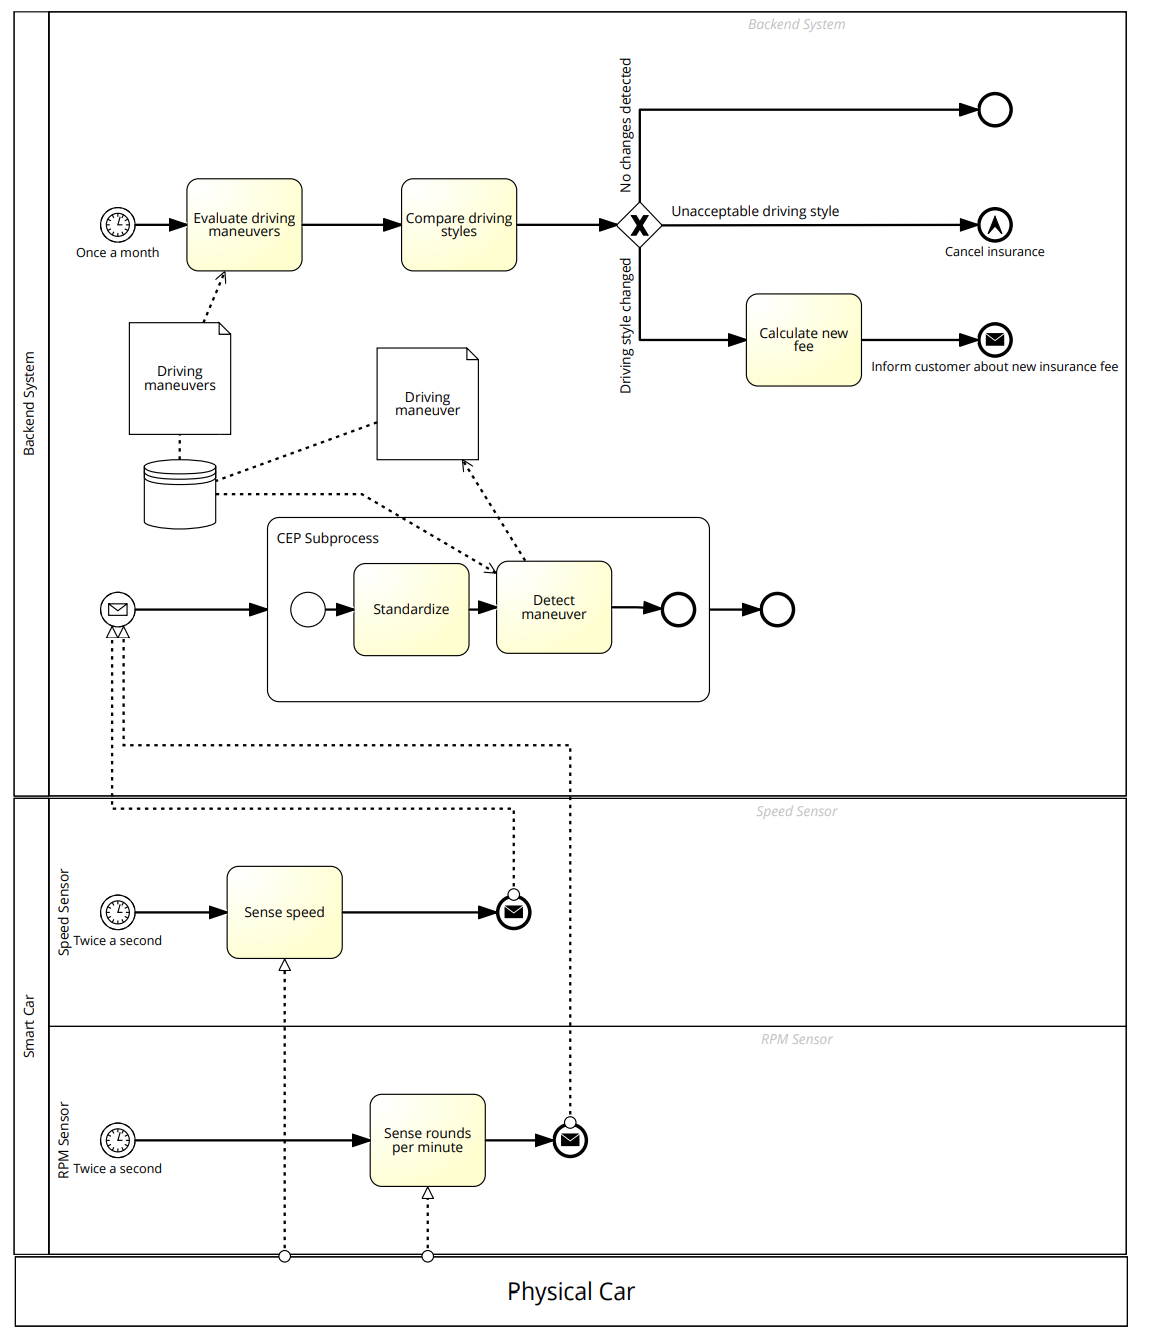
\includegraphics[height=17 cm,keepaspectratio,center]{figures/BPMNProcess}
	\caption{Darstellung des Prozesses zur Berechnung einer fahrstilbedingten Versicherungsrate mit BPMN}
	\label{fig:bpmnprocess}
\end{figure} 

\subsubsection{Darstellung nach IoT-A Konzept}
Der selbe Prozessablauf lässt sich durch die Hinzunahme der \ac{iota} Modellierungserweiterung in Abbildung \ref{fig:iotausecase} darstellen
\begin{figure}[H]
	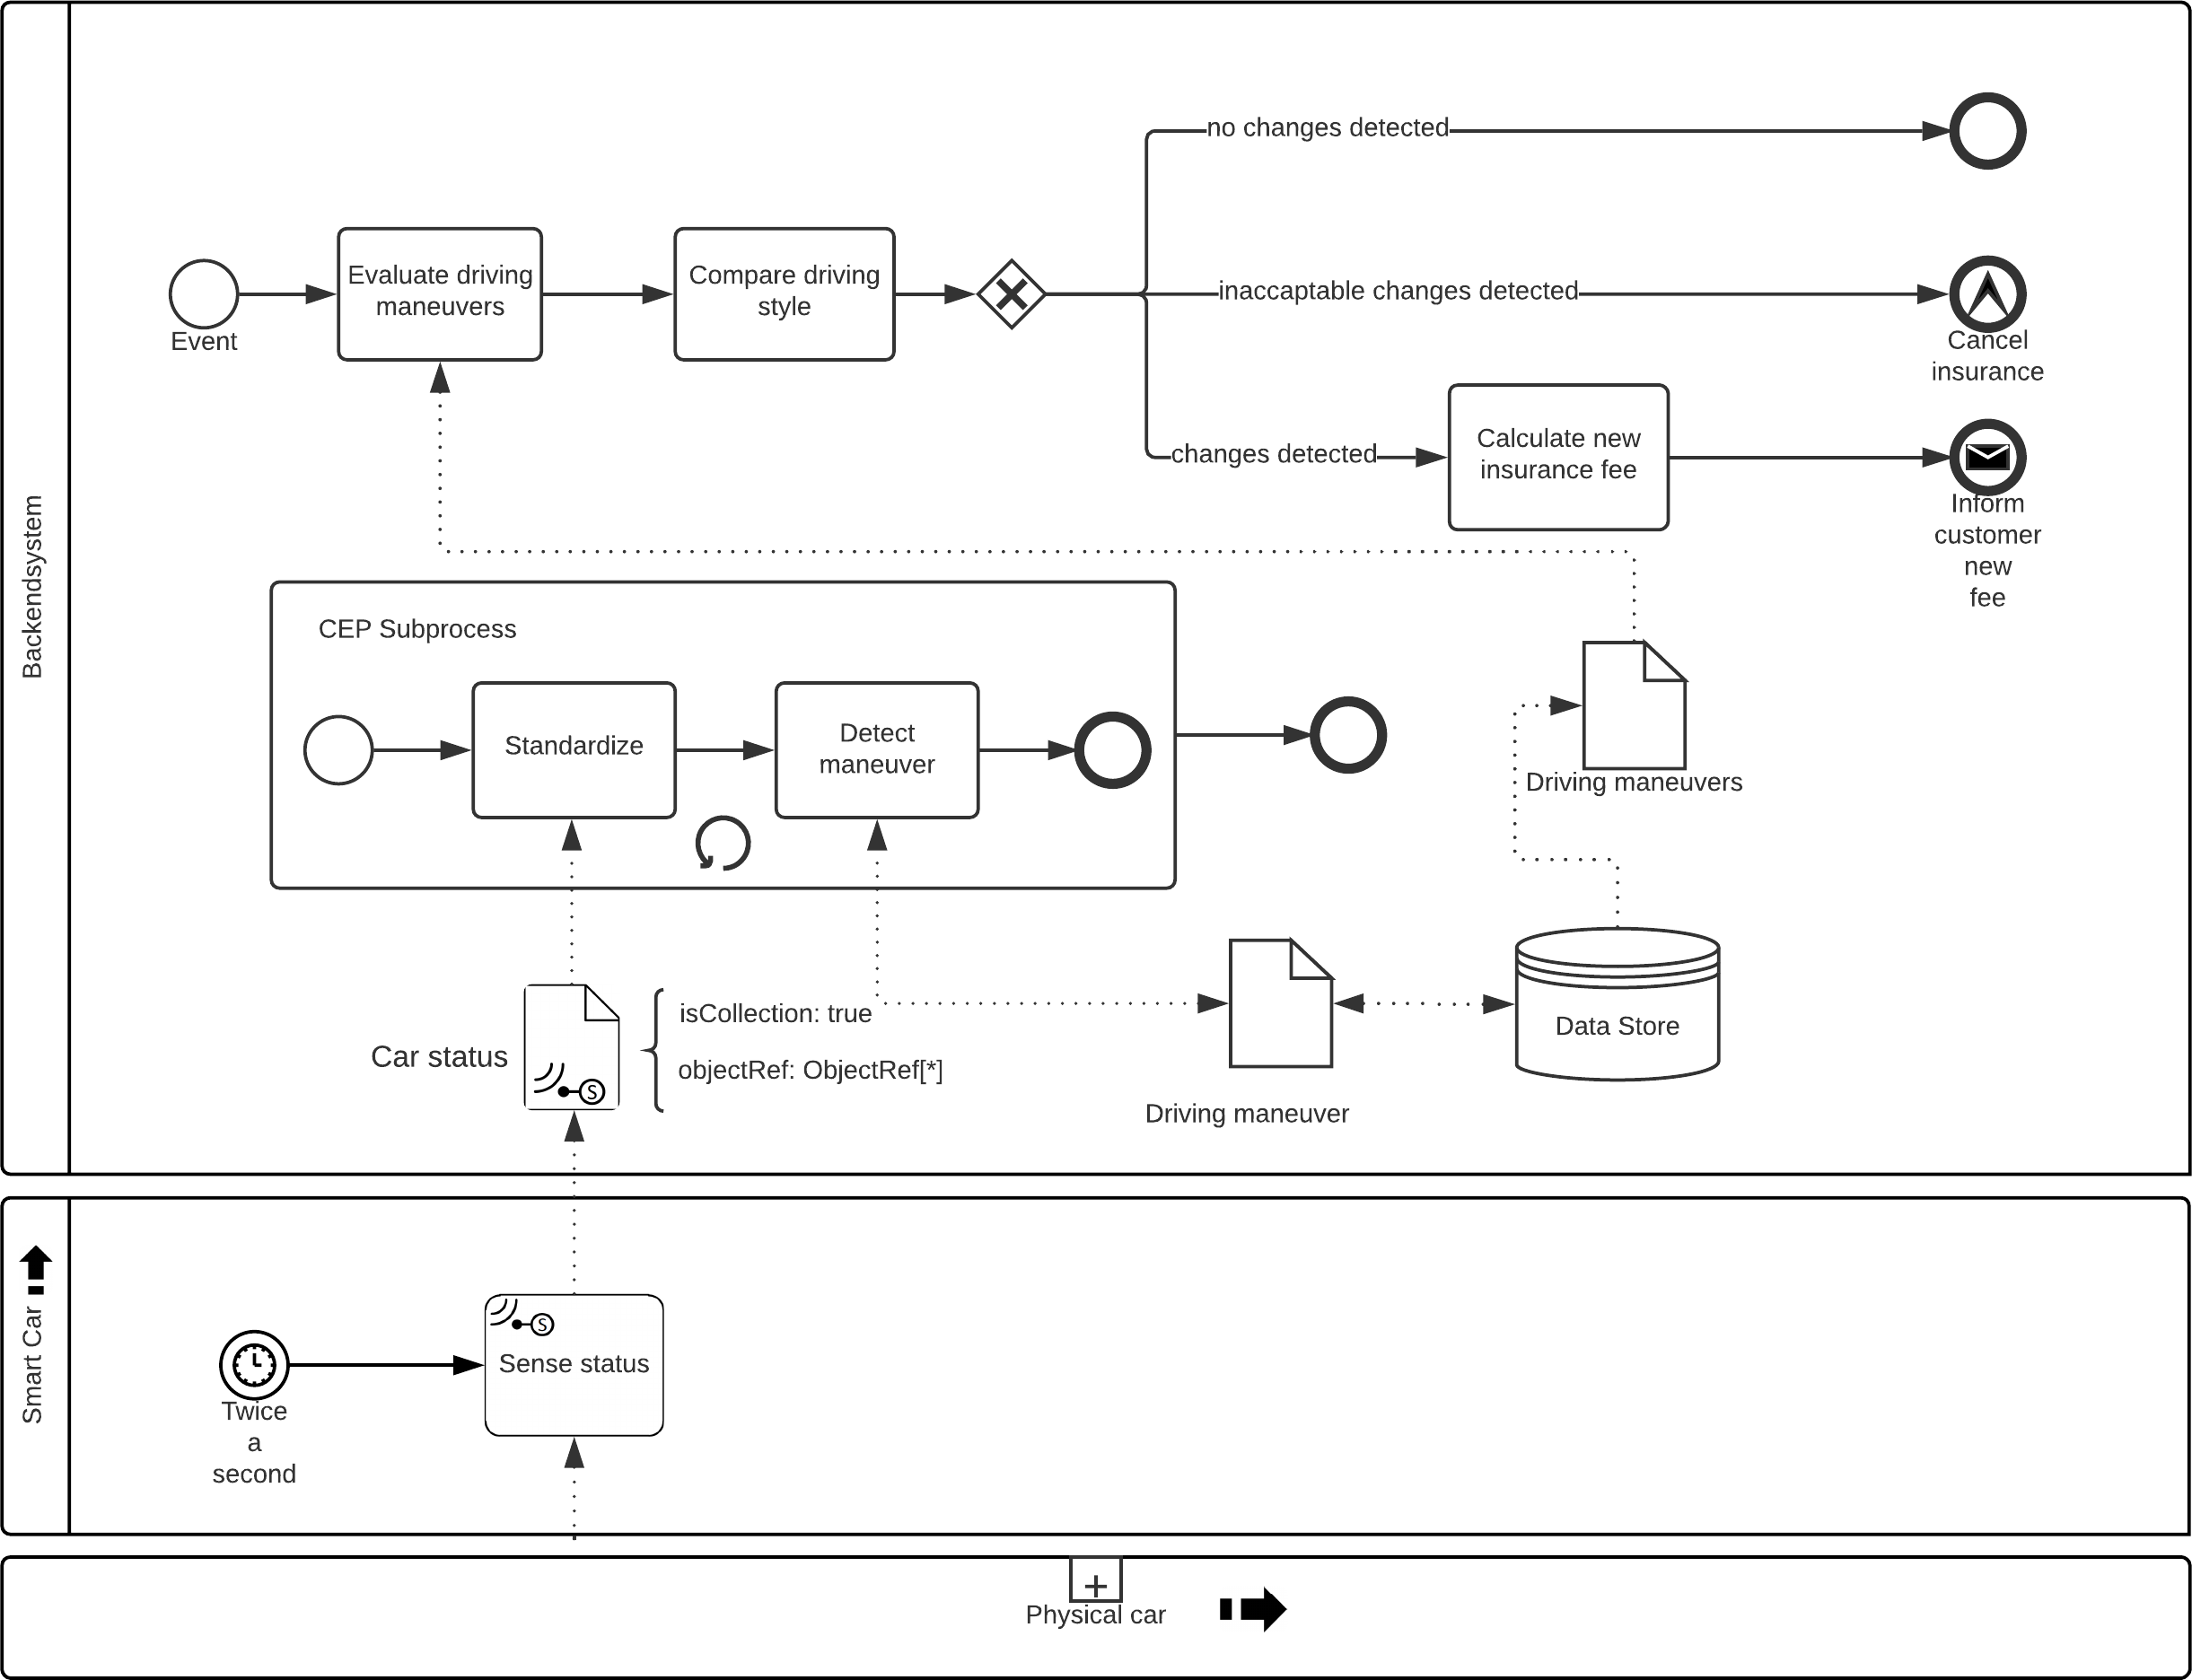
\includegraphics[height=12.5 cm,keepaspectratio,center]{figures/IoTAUseCase}
	\caption{Darstellung des Prozesses zur Berechnung einer fahrstilbedingten Versicherungsrate durch das IoT-A Konzept}
	\label{fig:iotausecase}
\end{figure} 

\subsection{Bewertung des Modellierungskonzeptes}
Das physische Auto wurde mit der Notation für mobile Prozessteilnehmer erweitert und besitzt weitere Parameter die im Schaubild zugeklappt sind. Durch diese Erweiterung des Prozessteilnehmers lassen sich bei der Umsetzung des Prozesses die  \ac{iot} Devices leichter dem \ac{eoi} in Form des physischen Autos  zu zuweisen was bei dem Standard \ac{bpmn} Prozessdiagramm nicht möglich ist.\\
Das smart Car stellt die Sammlung aller \ac{iot} Devices dar welche den Zustand des \ac{eoi} überwachen. Auch das Smart Car wurde als mobil gekennzeichnet, woraus Schlüsse über die Verfügbarkeit der Informationen gezogen werden können und somit einen Mehrwert gegenüber dem \ac{bpmn} Prozessdiagramm darstellt auch wenn dieser den \ac{iot} spezifischen Anforderungen noch nicht komplett entspricht.\\
Die \ac{iot} Devices führen die von dem \ac{iota} Modellierungskonzept entworfenen Sensing Task aus, welche eine Collection an Real World Data Objects erstellen. Diese Collection von Rael World DataObjects wird als einfaches Real World Data Object modelliert besitzt aber den Parameter isCollection sowie eine Liste an Referenzen zu den einzelnen Data Objects. Durch diese Darstellung lassen sich die erzeugten Informationen deutlich von DataObjects wie zum Beispiel dem Driving maneuver unterscheiden und lassen eine verständliche und einfache Weise der Modellierung zu ohne, dass dabei relevante Informationen verloren gehen. \\
Die referenzierten Real World Data Objects besitzen Definitonen über den Ort, Zeitpunkt, Produzenten sowie Angaben über ihre Qualität.\\

Das so erstellte Model entspricht bis auf den in Tabelle \ref{table:Evaluierung} bemängelten Aspekt der Mobilität den \ac{iot} spezifischen Anforderungen, da dieser lediglich eine Erweiterung um einen boolean Wert zum Standard \ac{bpmn} Prozessdiagramm darstellt. Somit bietet das \ac{iota} Modellierungskonzept eine bessere Basis für das Verständnis des Geschäftsprozesse und stellt dadurch einen Grundstein für die erfolgreiche Umsetzung des Geschäftsprozesses zu einem Workflow bereit.

\newpage
\section{Schlussteil}
Im Schlussteil dieser Thesis wird das Ergebnis des Inhaltes reflektiert, ein Fazit getroffen sowie weiterführende Arbeiten, Kritik und ein Ausblick gegeben\\

\subsection{Ergebnis}
Zu Beginn der Thesis wurden Grundlagen der Geschäftsprozessmodellierung, des \acl{bpm} und des \acl{iot} dargelegt. Im Bezug auf \ac{iot} wurden zusätzlich ein Domain Model festgelegt und  Grenzen zwischen den Arten von \ac{iot} Devices gezogen.\\
Anschließend wurden gängige Anwendungsgebiete des \ac{iot} untersucht um Muster in typischen \ac{iot} Workflows zu erkennen. Anhand dieser Muster wurden Unterschiede zwischen regulären Workflows und \ac{iot} Workflows definiert welche zu Anforderungen an die Modellierung von \ac{iot} Workflows definiert wurden\\
Anschließend wurden gängige Modellierungsmethoden und deren Erweiterungen auf die Verwendbarkeit zur Modellierung von \ac{iot} Workflows geprüft und mit den definierten Anforderungen evaluiert. Anhand der Evaluierung wurde die am besten für die Modellierung von \ac{iot} Workflows geeignete Modellierungsmethode ausgewählt.\\
Das auswählte Konzept wurde für die Modellierung eines vorgestellten \ac{iot} Workflows verwendet und daran Vorteile gegenüber der regulären Modellierungsmethode aufgezeigt.

\subsection{Fazit}
Durch die erweiterte Darstellungsmöglichkeit des von dem \acl{iota} Projekt bereitgestellten \acl{iapmc} ist eine sinnvolle Darstellung von \ac{iot} Prozessen möglich und die erweiterten Metadaten ermöglichen eine einfache Umsetzung des Geschäftsprozesses. Diese Metadaten ermöglichen es mit den standardmäßig vorhanden Business Rules engines auf die den \ac{iot} Devices genierten Events einzugehen und den Prozessfluss somit zu automatisieren.\\
Bei der Modellierung der Prozesse müssen jedoch stets die Funktionalitäten der einzelnen \ac{iot} Devices berücksichtigt werden, da diese für den Informationsfluss sowie dessen Verarbeitung beachtet werden müssen. So sind die in \ref{fig:iotdevices} dargestellten "Dumb Devices" lediglich in der Lage Daten zu sammeln und nicht auszuwerten, diese müssen also an einen weiteren Prozess Teilnehmer mitgeteilt werden welcher in der Lage ist die Auswertung der Daten und damit den weiteren Prozessablauf zu bestimmen übermittelt werden.\\
Generell ist es sinnvoll je größer ein Prozess wird mehrere \ac{iot} Devices in multi Sensor Gateways zu bündeln und ihre Aufgabe als Subprocess darzustellen um eine Bottom-Up Modellierung zu ermöglichen um somit einen Überblick über den Gesamtprozess zu ermöglichen. Wenn eine solche Sammlung von Devices zu Gateways nicht erfolgt ist keine Choreographie zwischen den \ac{iot} Devices selbst möglich sondern es findet eine Orchestration über das Backend statt.

\subsection{Weiterführende Arbeit/Ausblick/Kritik}
Wie kommen wir zu automatisierbaren Abläufen? -> Darstellung des Prozesses mit IoT-A und ausführung in BPMN Engine engies müssen IoT Spezifische Erweiterung akzeptieren\\
Workflow = automatisierte Ausführung von Business Processes

Problem, Nutzer müssen neue Technologie akzeptieren, Datenschutz Gesetze müssen international eingehalten werden. Häufig existiert die große Angst des "gläsernen" Konsumenten, diese führt dazu das sich viele Menschen trotz des Mehrwertes der neuen Geschäftsmodelle dagegen entscheiden um ihre Privatsphäre nicht zu verletzen. Hier gilt es Aufklärungsarbeit zu leisten und globale gesetzliche Rahmenbedingen für die Verwendung der \ac{iot} generierten Daten zu setzen.
\newpage

\addsec{Literaturverzeichnis}
\printbibliography[heading=none]
\newpage
\addsec{Anhang}

\end{document}
